%% 
%% Copyright 2019 Elsevier Ltd
%% 
%% This file is part of the 'CAS Bundle'.
%% --------------------------------------
%% 
%% It may be distributed under the conditions of the LaTeX Project Public
%% License, either version 1.2 of this license or (at your option) any
%% later version.  The latest version of this license is in
%%    http://www.latex-project.org/lppl.txt
%% and version 1.2 or later is part of all distributions of LaTeX
%% version 1999/12/01 or later.
%% 
%% The list of all files belonging to the 'CAS Bundle' is
%% given in the file `manifest.txt'.
%% 
%% Template article for cas-dc documentclass for 
%% double column output.

%\documentclass[a4paper,fleqn,longmktitle]{cas-dc}
\documentclass[a4paper,fleqn]{cas-dc}

%\usepackage[authoryear,longnamesfirst]{natbib}
%\usepackage[authoryear]{natbib}
\usepackage[numbers]{natbib}
\usepackage{listings}
\usepackage{adjustbox}
\usepackage{cleveref}
\usepackage{url}
\usepackage{wrapfig}

%%%Author definitions
\def\tsc#1{\csdef{#1}{\textsc{\lowercase{#1}}\xspace}}
\tsc{WGM}
\tsc{QE}
\tsc{EP}
\tsc{PMS}
\tsc{BEC}
\tsc{DE}
%%%

\begin{document}
\let\WriteBookmarks\relax
\def\floatpagepagefraction{1}
\def\textpagefraction{.001}
\shorttitle{SDN-Based Multidomain Service Provisioning and Topology Visualization}
\shortauthors{S. Barguil et~al.}

\title [mode = title]{SDN-Based Multilayer Multi-domain Use Cases from Topology Visualization to Service Provisioning}                      
%%\tnotemark[1,2]

%%\tnotetext[1]{This document is the results of the research
%%   project funded by the National Science Foundation.}

%%\tnotetext[2]{The second title footnote which is a longer text matter
%%   to fill through the whole text width and overflow into
%%  another line in the footnotes area of the first page.}%%

\author[1,4]{Samier Barguil}[type=editor,bioid=1]
\ead{samier.barguil@estudiante.uam.es}
\cormark[1]

\author[2]{Victor Lopez Alvarez}[bioid=2]
\ead{victor.lopezalvarez@telefonica.com}

\author[4]{Cristyan Manta-Caro}[bioid=2]
\ead{cristyan.manta@wipro.com}

\author[4]{Cristian Rosero-Carvajal}[bioid=10]
\ead{cristian.carvajal@wipro.com}

\author[2]{Arturo Mayoral Lopez De Lerma}[bioid=11]
\ead{arturo.mayoral@telefonica.com}

\author[2]{Oscar Gonzalez De Dios}[bioid=7]
\ead{oscar.gonzalezdedios@telefonica.com}

\author[3]{Edward Echeverry}[bioid=3]
\ead{edward.echeverry@telefonica.com}

\author[2]{Juan Pedro Fernandez-Palacios}[bioid=8]
\ead{juanpedro.fernandez-palaciosgimenez@telefonica.com}

\author[5]{Jutta Kemppainen}[bioid=5]
\ead{jkemppainen@infinera.com}

\author[5]{Janne Karvonen}[bioid=4]
\ead{jkarvonen@infinera.com}

\author[5]{Natalia Maya}[bioid=9]
\ead{nmaya@infinera.com}

\address[1]{Universidad Autonoma de Madrid, Madrid, Spain}
\address[2]{Telefonica I+D, Ronda de la Comunicacion, Madrid, Spain}
\address[3]{Telefonica Movistar, Transversal 60 No 114ª -55. Bogotá, Colombia}
\address[4]{Wipro Technologies Ltd., Doddakannelli, Sarjapur Road
Bengaluru - 560 035, India}
\address[5]{Infinera Corporation, 140 Caspian Court, Sunnyvale, CA 94089, USA}

\cortext[cor1]{Corresponding author}

%%\fntext[fn1]{This is the first author footnote. but is common to third
%%  author as well.}
%%\fntext[fn2]{Another author footnote, this is a very long footnote and
%%  it should be a really long footnote. But this footnote is not yet
%%  sufficiently long enough to make two lines of footnote text.}

%%\nonumnote{This note has no numbers. In this work we demonstrate $a_b$
%%  the formation Y\_1 of a new type of polariton on the interface
%%  between a cuprous oxide slab and a polystyrene micro-sphere placed
%%  on the slab.
%%  }


\begin{abstract}
Software-Defined Networking (SDN) is a powerful paradigm already transforming the everyday operations in Telecommunications Networks. SDN came with the idea of decoupling forwarding and control plane in the switches via OpenFlow, but it has evolved to cope with the needs of production networks. Network operators cannot change their footprint to upgrade the entire network to support SDN from scratch. This is why network operators adapt the original SDN concept into a hybrid SDN approach to have a pragmatic, evolutionary and economically viable solution. This paper tests an SDN architecture based on a hierarchical structure of SDN controllers for each technological domain and a Software-Defined Transport Networking (SDTN) controller, which deals with the end-to-end aspects of the service, topology, performance and inventory. Such a hierarchical approach allows a service provider to migrate islands in SDN domains, starting with the abstract programmatic interfaces and, when the devices support it, programming each device with a standard interface. 

Service provisioning is a key process in the value chain for supplying next-generation services to customers of all sizes and characteristics. Commonly, service provisioning was executed manually, then supported by service activator-tuned tools for the vendor-specific combination of network elements. With the advent of SDN, service delivery operations can be performed in an vendor-agnostic fashion using standard data models and protocols. However, new challenges persist, such as orchestrating multiple layers required for covering long-haul, medium and short distances. Multi-domain networking between IP/MPLS-based layers and underlying WDM multi-layer technologies require further coordination and orchestration. This paper presents the use cases to enable multi-domain service provisioning and the corresponding topology visualization. Moreover, this work relies on an hybrid SDN architecture combining the capabilities of the SDTN controller with Commercial Off-The-Shelf devices. 

\end{abstract}

% \begin{graphicalabstract}
% 
\includegraphics{figs/grabs.pdf}
% \end{graphicalabstract}

% \begin{highlights}
% \item Research highlights item 1
% \item Research highlights item 2
% \item Research highlights item 3
% \end{highlights}

\begin{keywords}
Software-Defined Networking,
\sep SDN-based Use Cases, 
\sep Service Provisioning,
\sep Multi-layer Topology,
\sep Network Modeling, 
\sep YANG,  
\end{keywords}

\maketitle

\section{Introduction}
SDN has emerged as the new reference paradigm to promote network automation and programmability. SDN has promoted the idea of a real transformation of all aspects of service delivery, network and traffic management. Mostly, because end-to-end automatic service provisioning, automated monitoring, fast issue detection and event-based decision taking are mandatory functionalities to offer a high-quality customer experience \cite{ordonez2017network,ong2017onf}. Similarly, Boucadair et all  \cite{boucadair2014software} refers to Software-Defined Networking as the ability to completely master the various components of the service delivery chain, so that the service that has been delivered complies with what has been negotiated and contractually defined with the customer.

Conceptually, SDN allows a full decoupling between control and forwarding plane on Physical Network Functions (PNFs) \cite{brief2014openflow}. This concept allows the centralization of complex tasks and enables the integration of white boxes (smaller equipment, high port density, low processing capacity, with generic hardware and lower production cost) in the network access layers. However, this promise is still not a complete reality. Although the term SDN seems quite new, more than twelve (12) have passed years since OpenFlow \cite{brief2014openflow} was defined and NICIRA was founded. NICIRA was the first company to develop a commercial SDN controller (NOX) \cite{gude2008nox,tavakoli2009applying}. Despite this and millionaire investments, today almost no service provider has a full operational SDN network deployed. Some of the main barriers found by service providers are:

\begin{itemize}
    \item There is still a lot of dependency on manually executed tasks.
    \item Network control tasks cannot be fully centralized.
    \item The stack of protocols deployed in the network is very complex.  The knowledge that network operators require to solve problems continues to be very specific.
    \item Confidence in automation solutions is not very high.
    \item Many networks have grown with the mix of companies, technologies and suppliers (e.g., a big one purchases a small one). 
   \item Standardization is not close; which generates a lack of complete interoperability between vendors.
\end{itemize}

New approaches have been released in order to take care of the above constraints and gradually adopt SDN. Some approaches have worked independently to close some of the standardization GAPS or enable the overlay SDN solutions. Others, promotes the combination of pure SDN controllers with programmable APIs to support both legacy and SDN ready-devices, to speed-up the SDN inclusion. The last kind of solution named as hybrid-SDN can support several scenarios. Mainly, the flavors differ between them in the Topology-role, the services supported, or the classes managed by each kind of device \cite{vissicchio2014opportunities}. Hence, based on the premise that Service Provider Networks, which rely on well know set of control plane protocols and a mixture of Commercial Off-The-Shelf devices needs hybrid SDN solutions to achieve programmability, the question that arises, and the scope of this paper, is on the approaches to present the network as an Application Program Interface (API) without breaking the existing network. 

Thus in this article, a field trial of a "Hybrid-SDN" architecture for a service provider is described. The trial includes a hierarchical control layer with multiple network controllers (one Hierarchical Transport Controller, two for IP/MPLS, and two for DWDM), as well as a real, operational multi-vendor commercial underlay network. This work test four use cases: three of them of multi-domain scenarios to validate the viability of the implementation of programmable network interfaces (APIs) in the control layer. The other one is a single domain test, focus on L2VPN provision. The paper also describes some of the main limitations found until now to deliver fully standard and interoperable solutions to enable the programmability in brownfield networks. 

The paper is structured as follows: \cref{section:arq} describes the SDN reference architecture tested named iFUSION. This architecture was defined to evolve Telefonica's transport network in the following years adopting the hybrid-SDN approach. Then, \cref{section:net} details the principles of network programmability including the concepts of YANG modeling and protocols used within the tests. \Cref{section:models} defines and differentiates service and device models. Additionally, the specific models used during the tests for IP/Optical service provisioning and topology collection are described too. Based on the models defined previously the \cref{sec:usecasesdef} describes the set of uses cases defined for this implementation. \Cref{section:trial} details the test architecture (based on iFUSION premises), including commercial network controllers and underlay network. In the end, \cref{section:results}  details the results obtained in this implementation. Finally, \cref{section:conclusions} resumes the conclusion of the present work and the next steps.

\section{SDN Architecture}
\label{section:arq}

There is not a unique way to enable the SDN in carrier grade scenarios. Until now, several options have been proposed \cite{bakshi2013considerations,karakus2017survey,birk2016evolving}. Some others, as the Google B4 has been successfully deployed \cite{jain2013b4}. However, based on the surveys done until now \cite{campbell1999survey,sinha2017survey,boucadair2014software} the reality of Network service provider industry is the lack of consensus on how to make the SDN automation premises completely real. In that sense, the "Hybrid-SDN" concept has arisen to describe three of the main gaps to be closed in the future network architectures: 
\begin{itemize}
    \item Coexistence: Refers to the heterogeneity in the infrastructure. It can be in the data plane (legacy and the SDN-ready devices), the control plane (NMS vs SDN Controllers), or both. 
    \item Communication: Conveys the idea of fully integration among fundamentally heterogeneous components of the network.
    \item Crossbreeding: Mainly indicates the degree of hybridization based on architectural trade-offs, for example: costs of transition, incremental deployment, easy of automation, among others. 
\end{itemize}

To cover those gaps, several conceptual architectures has been proposed \cite{vissicchio2014opportunities,vissicchio2017safe}. Some of them are part industrial definitions done within the consensus in standardization entities \cite{lee2015requirements}, others were created by the services providers itself. One of the most promising reference model is the \uppercase{iFUSION} architecture \cite{contreras2019ifusion}. iFUSION is based on the "controller-only" definition of \cite{sinha2017survey} to support network automation and programmability in a service provider environment. The \uppercase{iFUSION} main principles include the use of:
\begin{itemize}
    \item Standard North bound interfaces (NBI) leveraging \uppercase{RESTconf/YANG} \cite{bierman2017restconf}.
    \item Standard Configuration South bound interfaces (SBI) leveraging \uppercase{NETCONF/YANG} \cite{enns2011network}.
    \item YANG data models based on the latest developments of the standards development organizations (SDOs) \cite{bjorklund2016yang}: \uppercase{IETF}, \uppercase{ONF} and \uppercase{OpenConfig}.
\end{itemize}

As a complement to this architecture: APIs, Yang Data models and common protocols are defined as part of the i\uppercase{FUSION} program \cite{apistelefonica}. This definitionas are done in order to, describe the interaction of the control layer with the SDN devices in IP/MPLS + OPTICAL convergent Networks. 

The coexistence of legacy devices in the network is covered in the iFUSION architectural design. However the full integration and compliance relies more on the lack of adoption problem that in missing definitions.  Thus, until now, the acceptance of proprietary interfaces to configure the devices but common API interactions in the control layer (SDN Domain Controller and SDTN Controller) is the accepted solution to handle this drawback.

\begin{figure*}
	\centering
		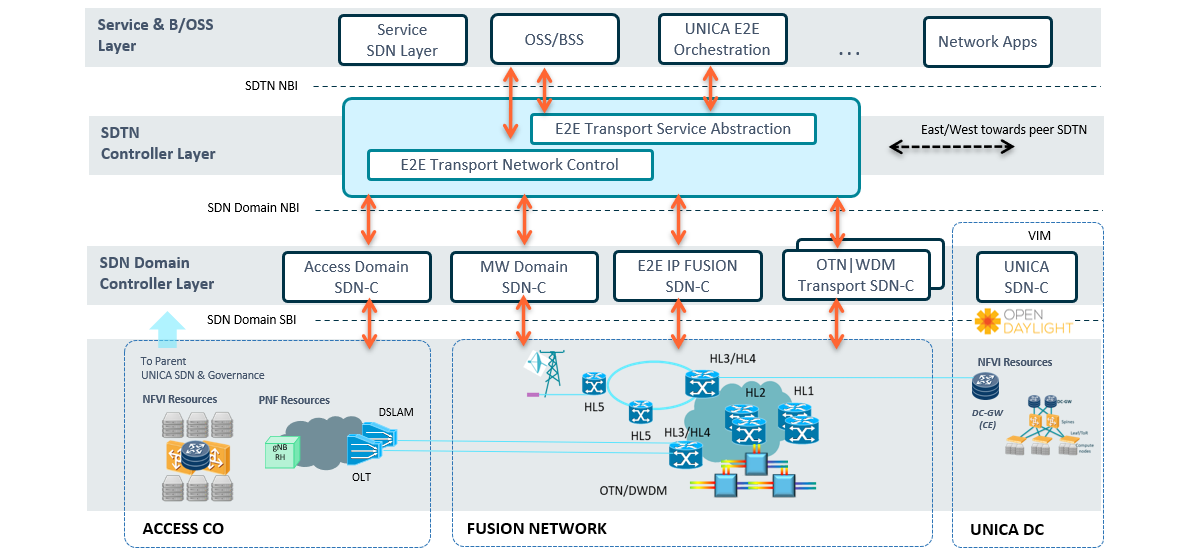
\includegraphics[width=\linewidth]{figs/ifusion_architecture.png}
	\caption{\uppercase{iFUSION} architecture}
	\label{FIG:1}
\end{figure*}
The i\uppercase{FUSION} architecture can be shown in terms of components and relationships among them in \cref{FIG:1}. Each of the architectural pillars are defined as:

\begin{itemize}
\item \textbf{SDN Domain}: A set of network elements under the supervision of the same SDN Controller. There are several possible levels in the decoupling of control and data planes. The preferred level of decoupling in Telefonica depends on the network technology. For example, in the case of MPLS, the network element runs the distributed protocols (e.g., IS-IS TE, RSVP-TE) and the controller only needs to configure it.

\item \textbf{SDN Transport}: The whole network controlled by following SDN principles. It is divided into SDN domains for technology/scalability/administrative principles. An SDN Transport Controller (also referred as an SDN Orchestrator) will take care of stitching the different domains/layers/technologies.

\item \textbf{SDN Domain Controller}: Is in charge of a set of network elements. It has standard southbound interfaces that depend on the technology, but not the equipment vendor, to communicate with the network elements. It also has a northbound interface to communicate with the SDN Orchestrator and the OSS.

\item \textbf{Software Defined Transport Network (SDTN) Controller}: Is in charge of providing services through several domains.. 

\item \textbf{Southbound Interface}: It is the interface, based on a standard, between the SDN domain Controller and the Network Element. Not only the communication protocol needs to be standard, but also the data model used.

\item \textbf{Northbound Interface}: It is the interface, based on a standard, between the SDN domain Controller and the OSSs and SDN Transport.

\item \textbf{Service SDN controller}: An additional SDN layer that takes into account services that might be needed. 
\end{itemize}

The \uppercase{iFUSION} architecture is designed as a hierarchical model where each network segment is controlled by a dedicated SDN domain controller. The transport network, due to its wide scope and complexity, is divided into three main technology domains: \hyperref[section:ip]{IP} domain and \hyperref[section:dwdm]{Optical} domain and MW domain.  

\subsection {IP domain}
\label{section:ip}
IP networks are deployed following a hierarchical model, mixing equipment from different vendors. The IP boxes are interoperable at both data and control plane levels (e.g., routing protocols such as IS-IS, OSPF or BGP). Due to scalability reasons, IP networks are typically subdivided into IP domains, so the routing and control protocols are confined to their administrative domains.

\begin{figure*}
	\centering
		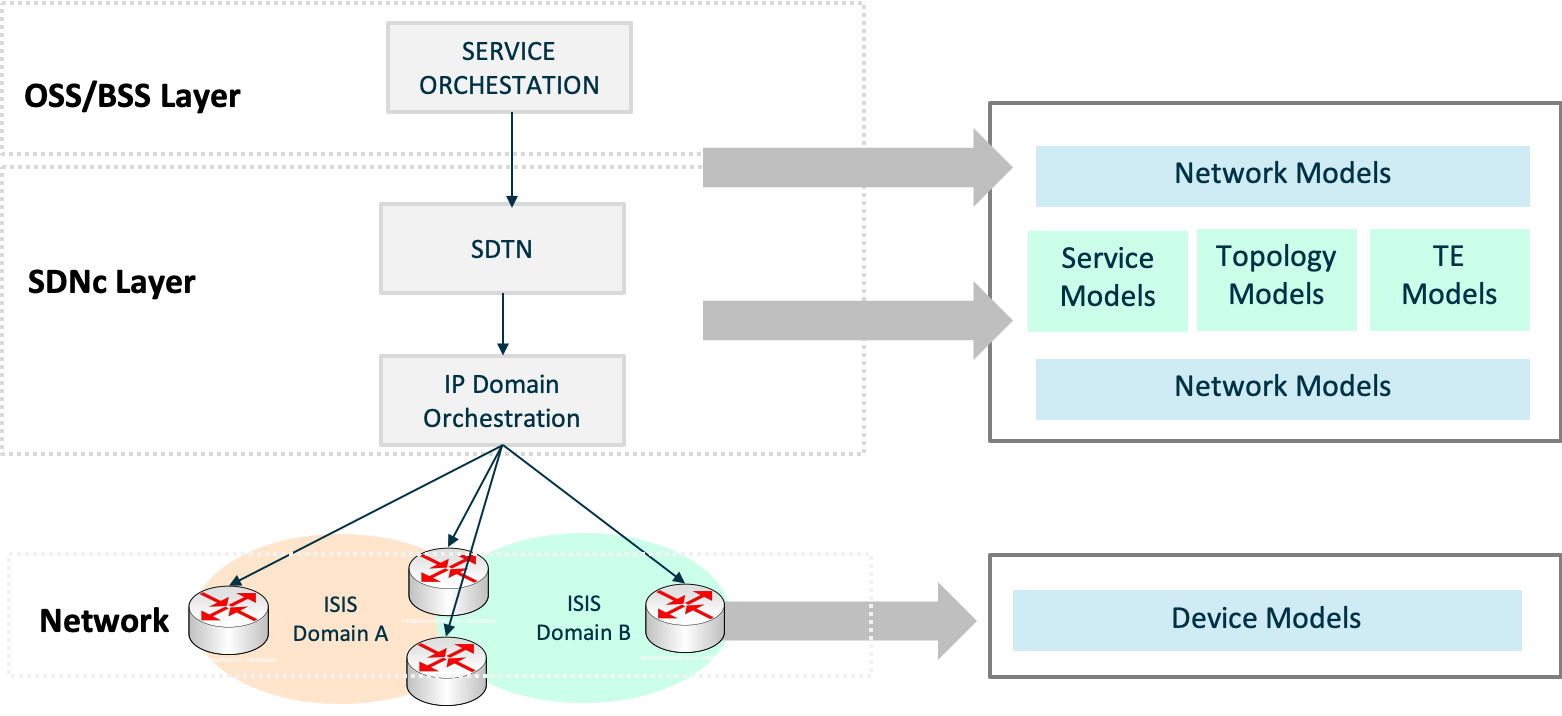
\includegraphics[scale=0.5]{figs/ifusion_multidomain_2.png}
	\caption{Single multi-vendor IP SDN-C deployment}
	\label{FIG:2}
\end{figure*}

The foreseen SDN solution for the IP segment is based on a single, multi-vendor IP SDN-C whose goal is to configure the IP network elements, as shown in \cref{FIG:2}. The target SBI for vendor-agnostic device configuration shall be compliant with NETCONF standard protocol. The set of device configuration data models are the ones defined in OpenConfig. 
The IP SDN-C shall perform TE and PCE tasks. With that purpose, some standard and mature control protocols, such PCEP and BGP-LS for MPLS networks, shall be implemented to complete the definition of the SBI. As a result, It is expected that the IP SDN controller will assume the control/management of:
\begin{itemize}
\item Device configuration of interfaces (VLANs) and routing protocols (BGP, ISIS, among others).
\item Traffic Engineering of MPLS tunnels (LSPs). 
\item Overlay network services (L2/L3 VPNs) device configuration (VRFs,\dots)
\end{itemize}

The IP SDN-C will be the main entry point to the network elements, to avoid overloading the elements and to provide a coherent view. The NBI of the controller will also be based on standard models defined in YANG and implemented on RESTCONF with JSON encoding. The NBI shall provide to higher entities within the SDN hierarchy:
\begin{itemize}
\item Device inventory information.
\item A layered topology view (L2/L3, MPLS) of its controlled network entities.
\item LSP provisioning and PCE.
\item Device abstraction for network services towards the SDTN, i.e., for overlay services VPNs (L2, L3)
\item Network state and performance monitoring information of the IP domain. 
\end{itemize}

\subsection{Optical domain}
\label{section:dwdm}
Transport WDM networks from different system vendors are deployed on a regional basis, either for technology redundancy, due to different optical performance requirements (metro vs. long-haul), or simply for commercial reasons. 

Without line-side interoperability of different WDM transceivers and Reconfigurable Optical Add-Drop Multiplexers (ROADMs), there is not a competitive advantage on a uniform configuration interface of the optical devices, since they cannot be mixed in a multi-vendor scenario, mainly because, both line systems and transceivers must be from the same vendor.

In the short term, Optical SDN-C are expected to provide network programmability and interoperability towards upper layers (multi-layer) and between vendors (multi-domain, multi-vendor), through the support of standard NBIs (i.e., coordination will be provided by upper layer hierarchical SDTN). This approach will enable the setup and tear down of connections in optical channels (OCh and ODU layers), the discovery of the network resources to compose a layered uniform view based on the OTN hierarchy, and the monitoring of the optical network.

The Hybrid SDN architecture proposed is compatible with a legacy control scenario where a distributed GMPLS control plane has been already deployed. GMPLS control plane can be centrally managed by an SDN domain controller by well-known and mature control protocols, such as PCEP, OSPF and/or BGP-LS, benefiting the gradual introduction of SDN. However, current NMS solutions shall evolve to, or coexist with, the SDN Controller model, enabling network programmability through its NBIs while keeping the current offered features for network creation, resource discovery and monitoring and service creation for L0/L1 layers. Standardization efforts targeting the definition of standard NBIs that can facilitate multi-vendor interoperability (by maintaining administrative domains for each vendor), such as ONF Transport API (T-API) \cite{lopez2016transport} and IETF models \cite{wu2017service}, are the more promising definitions for implementing such capabilities by abstracting the specific configuration of current distributed control planes embedded in Automatically Switched Optical Network (ASON) architectures. 
iFUSION relays on ONF Transport API 2.1 as the reference NBI for the SDN implementation in the optical transport segment, having been experimented on in several proof of concepts \cite{mayoral2016first,mayoral2017control,bravalheri2019vnf}. 

In the medium and long term, the direct programmability of the components can have interest in Point-To-Point, Metro and Regional scenarios, where disaggregation of optical transceivers and line side components can play an important role. In this line, OpenROADM \cite{oda2016learning,kundrat2019opening} and OpenConfig \cite{Openconfig,shaikhopenconfig} projects have already defined device configuration models for transponders and open line systems. Telefonica is approaching this transformation of the optical control in two phases:

\begin{enumerate}
    \item \textbf{Partial disaggregation}: As a medium-term objective, where the target is to define a standard interface based on NETCONF/YANG, which allows the Optical SDN-C to manage third-party terminal devices (i.e., transponders) that can transmit over the vendor line system.
    
    \item \textbf{Full disaggregation}: The long-term objective is the open management of the line system, i.e., the defragmentation of the optical transport network in vendor islands by the adoption of a common standardized interface for open line systems (multi-vendor) to be managed by a single optical SDN-C.
\end{enumerate}

\subsection{Integration of SDTN in the overall operator’s systems architecture}
\label{section:sdtn}
The SDTN Controller will keep visibility of all the transport network segments. It will expose an abstracted topology view of the network resources and the available set of network services to different clients through its Northbound APIs.  
One of the main drivers of deploying an SDTN controller is service automation. SDTN will enable it progressively, facilitating services and network configurations carried out manually today to become automated and available through this abstraction layer.  The level of abstraction can be different according to the needs of the northbound client (e.g., OSS, service orchestrators/SDN controllers, NFV orchestrator, etc.). 

The information exported through the NBI towards the OSS and other platforms will cover a number of functional areas. The service’s provisioning and network topology visualization within the Resource Lifecycle Management (RLM) domain will be the first set of functionalities adopted by the SDTN controller; tested in this paper. Progressively the SDTN will include Performance Management (PM) and Network Planning and Design (NPD), Fault Management (FM) and Resource Inventory Management (RIM) areas. The inclusion of these functional blocks is conditioned to the standardization of the required data models for the SDTN NBI and SDN-C SBI.

On the SBI of the SDTN, each technology Transport SDN-C shall expose vendor-agnostic network level programmability and resource discovery functionalities. The SDTN's SBI is intended, but not limited, to provide access to device configuration data, to expose per-OSI layer topology and network inventory information, and to offer active monitoring of device configuration changes and network state data (i.e., traffic statistics). 

\section{Network Programmability}
\label{section:net}

While the data plane technologies for transport networks have made significant progress in the last decades, the network management has lagged behind quite drastically \cite{claise2019network,edelman2018network}. Network Operators require highly train and skill network management professionals who are experts in the Command Line Interface (CLI) or Network Management Systems (NMS). 

With such tools at hand, developing new network services was a lengthy process that, in many cases, required the equipment vendor to develop additional functionality. Moreover, creating new behaviors in the network different of the ones envisioned exactly by the vendor was extremely complex regardless how small was the change.

This lack of manageability is often better understood when networking is compared with other technologies. For example, hypervisor managers, wireless controllers, IP PBXs, PowerShell and DevOps tools are part of the continuous integration and continuous development (CI/CD) in cloud providers \cite{mittal2017cloud,demchenko2016zerotouch}. Some of these are tightly coupled from a certain vendor, but others are more loosely aligned to allow for multi-platform management, operations and agility \cite{edelman2018network}.
The first attempt to break such rigidness and truly allow a programmability of a network was the birth of Software Defined Networking [SDN] aiming at decoupling the forwarding and the control plane. With protocols such as Openflow \cite{mckeown2008openflow} or Forces \cite{doria2010forwarding}, It is possible to program the per-packet behavior with a really high granularity. Later, P4 appears as a language to program in a platform agnostic way packet forwarding applications \cite{bosshart2014p4}. Those approaches are hard to scale at a service provider nation-wide (or international wide) scope and require a whole replacement of the network. Hence, Network Operators need to achieve programmability without needing to break existing network. So, It is a tradeoff between programmability and easiness to deploy. 

\subsection{Data models and abstraction}

The keys to network programmability are the use of well-defined data models and abstraction. The well-defined data models allow to represent any data that can be written or read, with a clear understanding of its format and possible values (if it is a string, an integer in a range, an address in the 4 octect format, etc) and its meaning.  The abstraction allows to work the right level of information. 

The low level can be found in the device-level APIs. For example, configuring ACLs (access control lists) allows to detail a per-packet behavior. Operators don’t expect to program the whole network with such fine detail, but for security reasons and user preferences, for some cases it is needed to go into such depths. In other case, the API will allow to configure and change the behavior of one of the control plane protocols running locally in a device.

A higher level of abstraction is achieved via the network-level APIs. In this case, the API provides the view of the whole network and allows queries and requests over it. In order to the network-level API to be effective, details of the device must be hidden. It must be taken into account that these network APIs are not just related to service provisioning automation (provisioning is a repetitive task and its components can be described in a technological way). The usage of APIs and programmatic interfaces goes beyond automation and offer much more than pushing configuration parameters.  It can be used to cover all FCAPs (Fault, Configuration, Accounting and Performance) capacities and Network planning tasks:
\begin{itemize}
    \item Network planning tasks if we include APIs to export distributed information such as the RIB, FIB and TE-Databases.
    \item Used to deploy closed-loop decision systems to take actions based on events reported by the devices.
    \item Automatically visualize the network relationships between the IP/MPLS and Optical packet transport domain, creating a common network view. 
 \end{itemize}   

Summing up, the set of envisioned APIs for network programmability are:
\begin{itemize}
\item \textbf{Network Service APIs}: The Service APIs provide a programmatic way of expressing the requirements of the service and general guidelines to deploy the service.
\item \textbf{Network topology APis}: Relation between the elements at different levels (layer 2, layer 3, IGP, UNI topology to expose client interfaces). 
\item \textbf{Traffic Enginnering API}: Allows to steer the traffic in the network by means of creating tunnels. 
 \end{itemize}
 
\section{Service Models}
\label{section:models}
Due to the network programmability necessities mentioned previously, protocols and Data models must be selected to allow the APIs definition. Those definitions limits the interaction between the different components, such as devices, network controllers, orchestrators and operation support Systems (OSSs). Recenlty, there has been great interest in the industry on using YANG as the universal language to define these data models. These data models can be easily converted into APIs with protocols such as Netconf or Restconf \cite{pugaczewski2017software}. 

This YANG-based set of definitions may include different groups of data models depending on the level of abstraction. One set, so called “device data models” is used strictly to model the behavior of devices (its hardware, logical configuration, protocols, etc). The other set, “service models”, are used to describe services in a portable way (independent of which network operator uses the model). This differentiation between Service and Device Models, introduced in early 2018, would allow the abstraction of some information in the control layer \cite{wu2017service}. As service is an overloaded term, in the context of this paper, we define a network service as: \textit{A set of device configurations that enables packets from a customer entering at selected locations in the network to reach other locations following a desired behavior)}. These services are for example layer 3 VPNs or layer 2 VPNs. 

There are two types of service models to consider:
\begin{itemize}
\item 	\textit{A customer service model}: Captures the characteristics and requirements of the service solely from the customer point of view. For example, the requirements in terms of latency and bandwidth between customer locations are part of the service definition. The customer service model describes the location of the customer sites and a reference to its entry point in the service provider network. However, as the customer service models are intended to be consumed by the customer of the network, all internal details are hidden. The customer service models are hence aimed at being consumed by the service orchestration layer. Examples of customer service models are L3SM \cite{rosen2006rfc} and L2SM \cite{wen2018yang}.

\item 	\textit{Network Service Models}:  Describes the service from the point of view of the service provider network. The Network Service models, in addition, capture the nodes in the network where the service needs to be delivered, without requiring intermediate translations and the real interfaces into which the customer traffic is received. Programmatically, new end points can be easily added and removed. The behavior at the interface, both per packet and in terms of routing can be programmed. Finally, the preferences on the underlay transport, that is how packets are sent between the edge packet devices, can also be expressed.
\end{itemize}

Example of network service model definitions used during this implementation are described in \Cref{section:IPmodels} for IP and \cref{section:OPTmodels} for Optical.

\subsection{IP Network Models}
\label{section:IPmodels}

The IP service models used in this work, are YANG modules defined to: First support the creation, deletion and retrieval of \hyperref[section:l3nm]{L3} or \hyperref[section:l2nm]{L2VPN} services and Second, collection of the IP/MPLS network \hyperref[subsection:IPtopo]{topology}. As detailed before, the models used are the result of a collaborative effort inside the standardization entities, in this particular case the IETF.

\subsubsection{L3NM}
\label{section:l3nm}
The Layer 3 Virtual Private Network (VPN) service defined in RFC 4364 \cite{rosen2006rfc} provides a multipoint, routed service to the customer over an IP/MPLS core. The L3VPNs are widely used to deploy 3G/4G, fixed and B2B enterprise services principally due to the fact that not only several traffic discrimination policies can be applied across the transport network but also because several stitching methodologies can be configured to combine access and transport services. 

Some service models have been defined and standardized until now to support L3VPN creation. The first one, was the L3SM \cite{rfc8299}. L3SM is a Customer Service Model that describes the requirements of an L3VPN service based on the customer requirements; the L3SM model keeps some commercial parameters as the customer site location.

L3NM \cite{voyer2019internet} is a complementary Network Model of the L3SM. It differs from the L3SM because it is completely network centric. It focus only in the service provider's internal network configurable parameters delegating the customer information to the L3SM. Additionally, the L3NM can be exposed by network controllers to manage and control the VPN Service configuration in multi-domain scenarios. It contains information on the service provider network such as an identifier of each network element in the IP/MPLS domain (NE-ID) and the interface identifier. It allows the dynamic network resources management, such as the auto-assigment of Route Targets (RTs) or Route Distinguishers (RDs).

The \cref{FIG:l3nm}a shows the structure of the L3NM YANG data model. It has a  main container (L3NM) used to group the information of the VPN-Service (VRFs) and the Site-Network Accesses (Logical Interfaces). Complementary containers are defined to have the relationship of the logical and physical infrastructure. For example, the Site-Bearer was defined to relate the Logical Interfaces to the physical ports assigned in for the service. The IE-Profiles stores the Import/Export policies.  

The L3NM model is used in this field trial as the data model between the SDTN and the IP SDN-C. The SDTN includes network-specific information in the service request (i.e., transport LSP binding, routing profiles or encryption); to facilitate multi-domain orchestration, the SDTN assigns some logical resources (RTs and RDs) that must be synchronized between domains.

\begin{figure*}
	\centering
		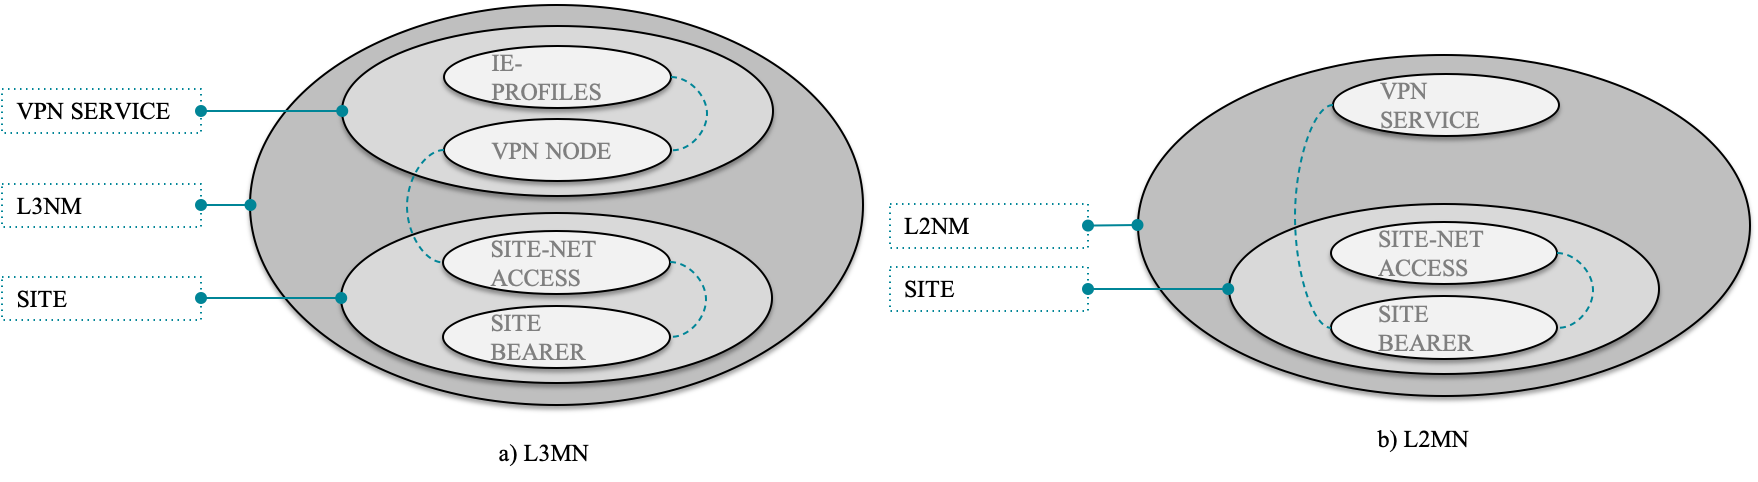
\includegraphics[scale=0.55]{figs/L3NM_L2NM.png}
	\caption{L2NM and L3 Data model structure}
	\label{FIG:l3nm} 
\end{figure*}

\subsubsection{L2SM}
\label{section:l2nm}

L2 services belong to the class of IP virtual leased line services (VLLs) or virtual private LAN services (VPLS)\cite{andersson2006framework}, which are a fundamental part of the service portfolio offered by SPs. VLLs and VPLS can be generally described as point-to-point and point-to-multipoint solutions respectively. In the same way as the L3SM is the service model proposed for L3VPNs, there is already an equivalent for L2 services. This model is named L2SM \cite{wen2018yang}. 

As with the L3, the L2SM is a customer centric model. It has two main containers: the VPN Service and the site depicted in \cref{FIG:l3nm}b. The VPN-Service container has all the technological parameters of the services that is going to be deployed, for example: service type (i.e., bgp-vpls, pw3, ldp-vpls, \dots) or service topology (i.e., p2p, p2mp). The site container has all the customer information, including the customer location and the connectivity parameters between the CE and the PE. It has a Site-Bearer container to relate the logical interfaces with the physical infrastructure assigned for the service deployment.

This model misses some specific network configuration, which needs to be stored or derived by the network controller to deploy the final configuration on the network devices. Additional work to complement this model can be proposed for future implementations.  

\subsubsection{Network Topology}
\label{subsection:IPtopo}

The proposed control architecture relies on providing different levels of abstraction for each control layer. Therefore, the needs in terms of topology and knowledge of the service provider network differ among components. 

Network topology is an abstract representation of the physical nodes, links and network interconnections. It is crucial to get and graphically represent network information, such as:
\begin{itemize}
    \item Structure (Connectivity and Paths).
    \item Performance (Available bandwidth per link).
    \item Availability of physical and logical resources.
\end{itemize}

Currently, the topology representations are limited to the scope of each of the network vendors i.e., each NMS has its particular/proprietary network view. Sometimes Dummy devices from a third party can be included to simulate the interconnection of the networks. However, nowadays obtaining a unified view of the entire IP network is not possible.

However, as part of the I2RS working group in the IETF, a common base model for an initial network topology representation has been defined. The model includes Nodes and Links. As a complementary work, several augmentations have been done to cover the L2, L3 and TE functionalities.

In this implementation, the topology models used to retrieve the IP network are: 
\begin{itemize}
\item IETF Network (RFC8345): Includes the Network, Node and Link concepts \cite{clemm2018yang}.
\item IETF Network Topology (RFC8346): Includes Termination Points inside the Nodes and IP specific parameters such as addressing information \cite{varga2018internet}.
\end{itemize}

\subsection{Optical Network Model}
\label{section:OPTmodels}

In this section, the standard reference model use for the control/management of networks based on WDM/OTN technologies is described. The proposed solution for the Optical SDN-C's NBI is based on ONF T-API information models, as described previously.  NBI message transportation is performed using the RESTCONF protocol. Please note that in this transport domain, the same solution (T-API + RESTCONF) is also proposed to be the NBI of the hierarchical SDTN Controller towards the Service B/OSS layers.

\subsubsection{Provisioning}

\begin{figure*}
	\centering
		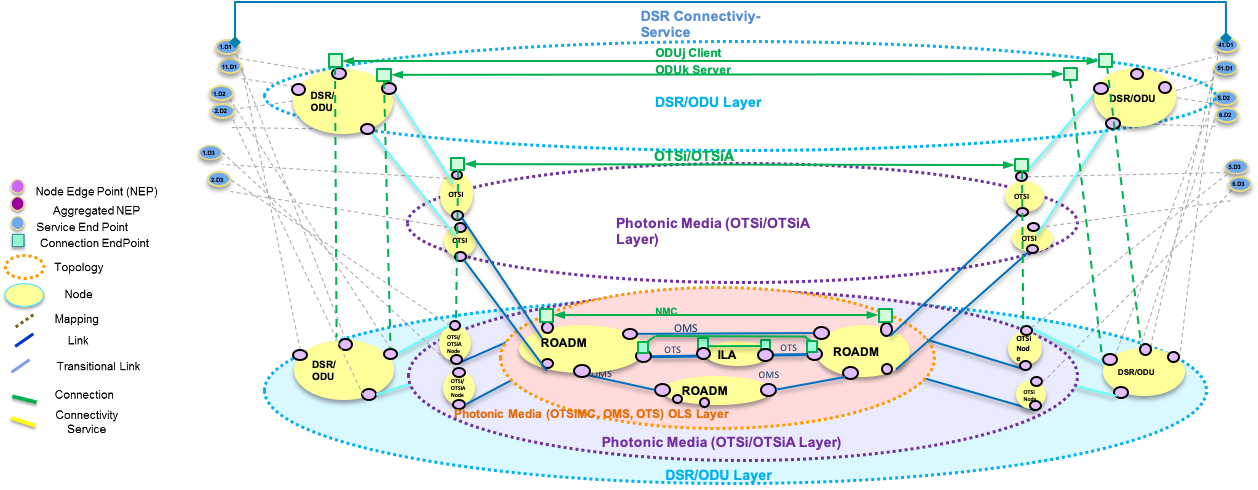
\includegraphics[scale=0.8]{figs/ONF-T-API.png}
	\caption{Multi-layer topology and connectivity models based on ONF T-API}
	\label{FIG:ONF-T-API}
\end{figure*}

The connectivity provisioning into the WDM/OTN optical layers is strictly related with the model proposed. \Cref{FIG:ONF-T-API} represents the optical network topology arrangement proposed in the previous figure and the multi-layer hierarchical connectivity modeling that is being detailed in this section.

The connectivity model introduces two central concepts: on one hand, the tapi-connectivity:connectivity-service object models intentionally solicited by the T-API client layer to be deployed into the network, and on the other hand, the tapi-connectivity:connection objects that represent the actual adjacencies between logical interfaces created by configuring the network, or in brief, the connectivity configurations in the network. 

The network model is multi-layer, so it is needed to establish multi-layer relationships into the model. These relationships are constructed by the relationship between Logical Termination Points (LTPs), which in T-API are modeled as two different objects: 
\begin{itemize}
    \item The \textbf{Node-Edge-Points} (NEPs) which represent the resources available at a given layer LTP to provide connections.
    \item The \textbf{Connection-End-Points} (CEPs) that consume part of all of the NEPs’ exposed resources to create the connections between different points of the network.
\end{itemize}

In our proposed reference implementation, we distinguish between two different level of connections:

\begin{itemize}
    \item \textbf{Cross-Connections (XC)}: defined as connections between Connection-End-Points of the same layer within a Forwarding-Domain (represented as a\\ \texttt{tapi-topology:node} object). 
    \item \textbf{Top Connections}: defined as end-to-end connections between CEPs within the same layer, which may span multiple Forwarding-Domains. Top connections are composed of zero or more XCs that belong to the same layer of the Top Connection.
\end{itemize}

Then, the multi-layer relationships are constructed by stacking CEPs over NEPs and providing the upper layer resource representations by the dynamic creation of new NEPs, e.g., an OTSi connection, when created and operational, provides the ODU upper layer resources in the form of NEPs, which in turn can be consumed to create ODU connections that will provide the DSR layer resources.

\subsubsection{Topology}
\label{subsection:OPTopo}

The topology model should provide the explicit multi-layer topology representation of the L2-L0 network, including OTS, OMS, MC, OTSIMC, OTSi/OTSiA, ODU and DSR layers. The network logical abstraction collapses all network layers (DSR, ODU, OTSi/OTSiA and Photonic Media (OTSiMC, MC, OMS, OTS)), which are represented explicitly into a single topology (T0 – Multi-layer topology), modeled as a \texttt{tapi-topology:topology} object within the: \\
\texttt{tapi-topology:topology-context/... \\
... tapi-topology:nw-topology-service} and \\ \texttt{tapi-topology:topology-context/topology}. 

The T0 – Multi-layer topology MUST include:

\paragraph{DSR/ODU Layers:}
DSR/ODU forwarding domains are represented as multi-layer and multi-rate \texttt{tapi-topology:node}, allowing the representation of the internal mapping between DSR and ODU NEPs (multi-layer) and multiplexing/demultiplexing across different ODU rates (multi-rate). 

The DSR/ODU layer network MUST be represented explicitly at the lowest partitioning level, i.e., each DSR/ODU forwarding domain MUST be represented as a single tapi-topology:node. The following network components included within the category of ODU forwarding domain are:

\begin{itemize}
    \item Transponders.
    \item Muxponders.
    \item OTN switching nodes connecting client and line boards.
\end{itemize}

\paragraph{OTSi/Photonic Media layers:}
The OTSi layer represents the optical side of the optical terminals (transponders/muxponders). This layer consists of nodes representing the mapping and multiplexing of OTSi signals. It consists of nodes including OTSi client end-points representing the Trail Termination Points (TTPs) of the OTSi connections and OTSi/OMS end-points representing the physical connectivity with ROADM/ Fixed Optical Add Drop Multiplexers (FOADM) add/drop ports.

DSR/ODU and OTSi layers may be collapsed into a single multi-layer node or split into two logical node representations by using the Transitional links concept to represent the potential layer transitions between ODU and OTSi.

\paragraph{Photonic-Media layer:}
The Photonic-Media layer models the Optical Line Protection (OLP) components, the ROADMs/FOADMs and In-Line Amplifier (ILAs) network elements. Moreover, all the lowest photonic connectivity is represented as PHOTONIC\_MEDIA \texttt{tapi-topology:link} objects collapsing the OTS/OMS layers and allowing the placement of specific monitoring OAM functions of these layers. These forwarding domains SHALL expose the capability to create Media Channel connection and connectivity services between its end-points.

\begin{figure}
	\centering
		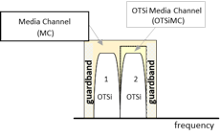
\includegraphics[scale=0.75]{figs/Media_channel.png}
	\caption{Media-channel entities relationship}
	\label{FIG:Media_channel}
\end{figure}

Moreover, the Media Channel layer represents the available resources for the reservation of spectrum resources for a given OTSi channel. The concatenated reserved portion of a route is represented as a Media-Channel (MC) construct, and by the OTSiMC construct, which represents the actual portion of the spectrum occupied by the signal (MC spectrum must be wider than the OTSiMC). These modeling concepts are critical for the realization of the Open Line System concept introduced by the partial disaggregation of the optical networks. See \cref{FIG:Media_channel} graphical representation for more clarity.


\section{Use Cases Definition}
\label{sec:usecasesdef}
Based on the service models described previously in \cref{section:models} and using the iFusion Network architecture as a target (\cref{section:arq}), two end-to-end use cases were defined for testing in this work: 
\begin{itemize}
    \item Multi-domain IP L3VPN provisioning
    \item Multi-layer Topology Discovery \& Visualization
\end{itemize}
Derived from the multi-domain use cases, additionally the single domain provision use cases where also defined:
\begin{itemize}
    \item Single-domain IP L2VPN provisioning
    \item Single-domain Optical provisioning
\end{itemize}

The details covered on each of the use cases are described in the following subsections:

\subsection{Multi-domain IP L3VPN provisioning}
\label{section:muli-l3nm}

As described previously in the \cref{section:l3nm}, the L3VPN services are not exclusive of single domain implementation. Multi-domain IP L3VPN is a common requirement in service providers. As the reality of service provider networks implies the coexistence of multiple AS, multiple IGPs, or multiple vendor network segmentation. Additionally, even if the iFusion architecture depicted in \ref{FIG:1} defines only one controller for the entire IP network, the lack of common models support on the network layer derives in the requirement to temporally expand it to support several IP-SDNcs. So this use case the service provisioning process requires a set of interactions between the SDTN and more than one IP SDN-C.

In that sense, the scope of this work includes two domains within the same IP/MPLS network. Each domain is controlled by an independent SDN-C \ref{FIG:field_trial_ip}. Each controller has implemented the IETF L3NM model described in subsection \cref{section:l3nm}. So at the end, the goal of this use case is to prove the SDTN capacity to:
\begin{itemize}
    \item \textbf{Create}, \textbf{Modify} and \textbf{Delete}: Delegate the required provision parameters to each controller in order to Create services in an operative multidomain IP/MPLS network.
    \item \textbf{Retrieval}: Get the service information from each controller and expose the services with an unified view of it.
\end{itemize}

\begin{figure}
	\centering
		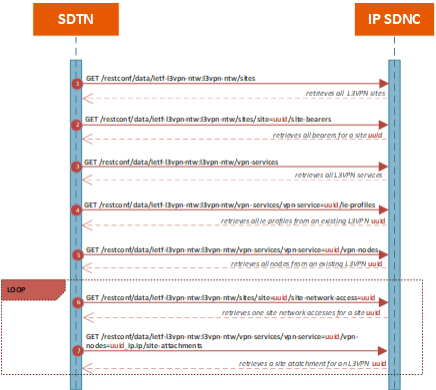
\includegraphics[width=\linewidth]{figs/l3vpn_workflow.png}
	\caption{Messages Interchanged for IP multi-domain L3VPN service creation.}
	\label{FIG:l3vpn_workflow}
\end{figure}

The information exchanged between the SDTN and the IP-SDNc are limited by the yang data model definitions. Thus, as depicted in \cref{FIG:l3nm}a each of the containers of the L3NM must be implemented in the control element to support the specific RESTCONF operation. Specific and stadard RESTCONF paths must be supported too. In that sense, the following four steps are needed to provision a multi-domain L3VPN service:
\begin{enumerate}
    \item Create Site:
    \item Create Bearer:
    \item Create VPN-Node:
    \item Create Site-Network-Access:
\end{enumerate}

\Cref{FIG:l3vpn_workflow} depicts the workflow used by the SDTN to create the services on the IP SDN-Cs. Each creation (POST) operation is complemented by the retrieval (GET) operation with their corresponding RESTCONF paths. 

%\begin{figure}
%	\centering
%		\includegraphics[width=\linewidth]{figs/multidomain_service_provisioning%_workflow.png}
%	\caption{Workflow for multi-domain service provisioning SDTN-SDN-C}
%	\label{FIG:multidomain_service_provisioning_workflow}
%\end{figure}

\subsection{Multi-layer Topology Discovery \& Visualization}

The multi-layer topology use case is based on the data provided by all the \hyperref[subsection:IPtopo]{IP} and \hyperref[subsection:OPTopo]{Optical WDM/OTN} SDN-Cs. The scope of it includes the composition of multiple sources and data formats (i.e., IETF context for IP or T-API context for Optical) to create a common view of the network. The models used to create the multi-layer topology are:
\begin{itemize}
    \item For the optical domain representation: Topology and Connectivity Service modules. These models provide information for layers from L0 to L2.
    \item For the IP/MPLS domain representation: The IETF\\ \texttt{ietf-network:networks} is the basis to expose the network model (nodes and IP Links) and the \\ \texttt{.../node/nt:termination-point} are used to expose the Termination points (Ports) of a specific node.
\end{itemize}
    
Additionally, a correlation parameter is defined to join the IP and Optical layers. We have denoted this parameter as the \texttt{Plug-id}. This additional definition is needed due to there being no dynamic protocol or common element between the ONF/IETF standards that would allow their direct correlation. The \texttt{Plug-id} parameter is added in the IETF termination points and in the T-API connectivity services. 

It is necessary to remark that in the T-API model, the \texttt{Plug-id} parameter is a "String," while in the IETF model it is "Binary;" therefore the SDTN MUST have the ability to translate the “Binary” value to “String” or vice versa to be able to make the match in the correlation process considered to be standardized.

To fill the \texttt{Plug-id} attribute automatically between the layers, it is required that the SDTN performs a process based on meta-heuristic algorithms in which the performance data at a termination-points level, both in the IP and Optical layers, will be correlated. Clock \& Time must be perfectly synchronized between the Tx/Rx points bidirectionally. Meta-heuristics must include the geo-location parameter of the nodes as input. However, the design of this process is currently under study and is based on real-time information that can be delivered by the telemetry engines.

\begin{figure}
	\centering
		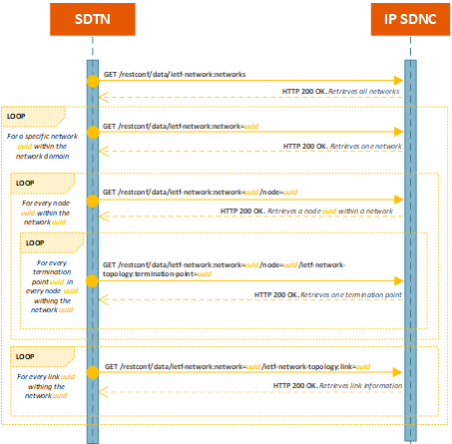
\includegraphics[width=\linewidth]{figs/ip_topology_workflow.png}
	\caption{Messages Interchanged for IP Topology Discovery between the SDTN and IP SDN-C}
	\label{FIG:ip_topology_workflow}
\end{figure}

Starting with the optical domain, a set of T-API version 2.1 queries were sent in order to build the topology by extracting the list of networks as well as topology details such as nodes, links, connections and service interface points available. The query exchange process is shown in the UML diagram depicted in \cref{FIG:optical_topology_workflow}.  

\begin{figure}
	\centering
		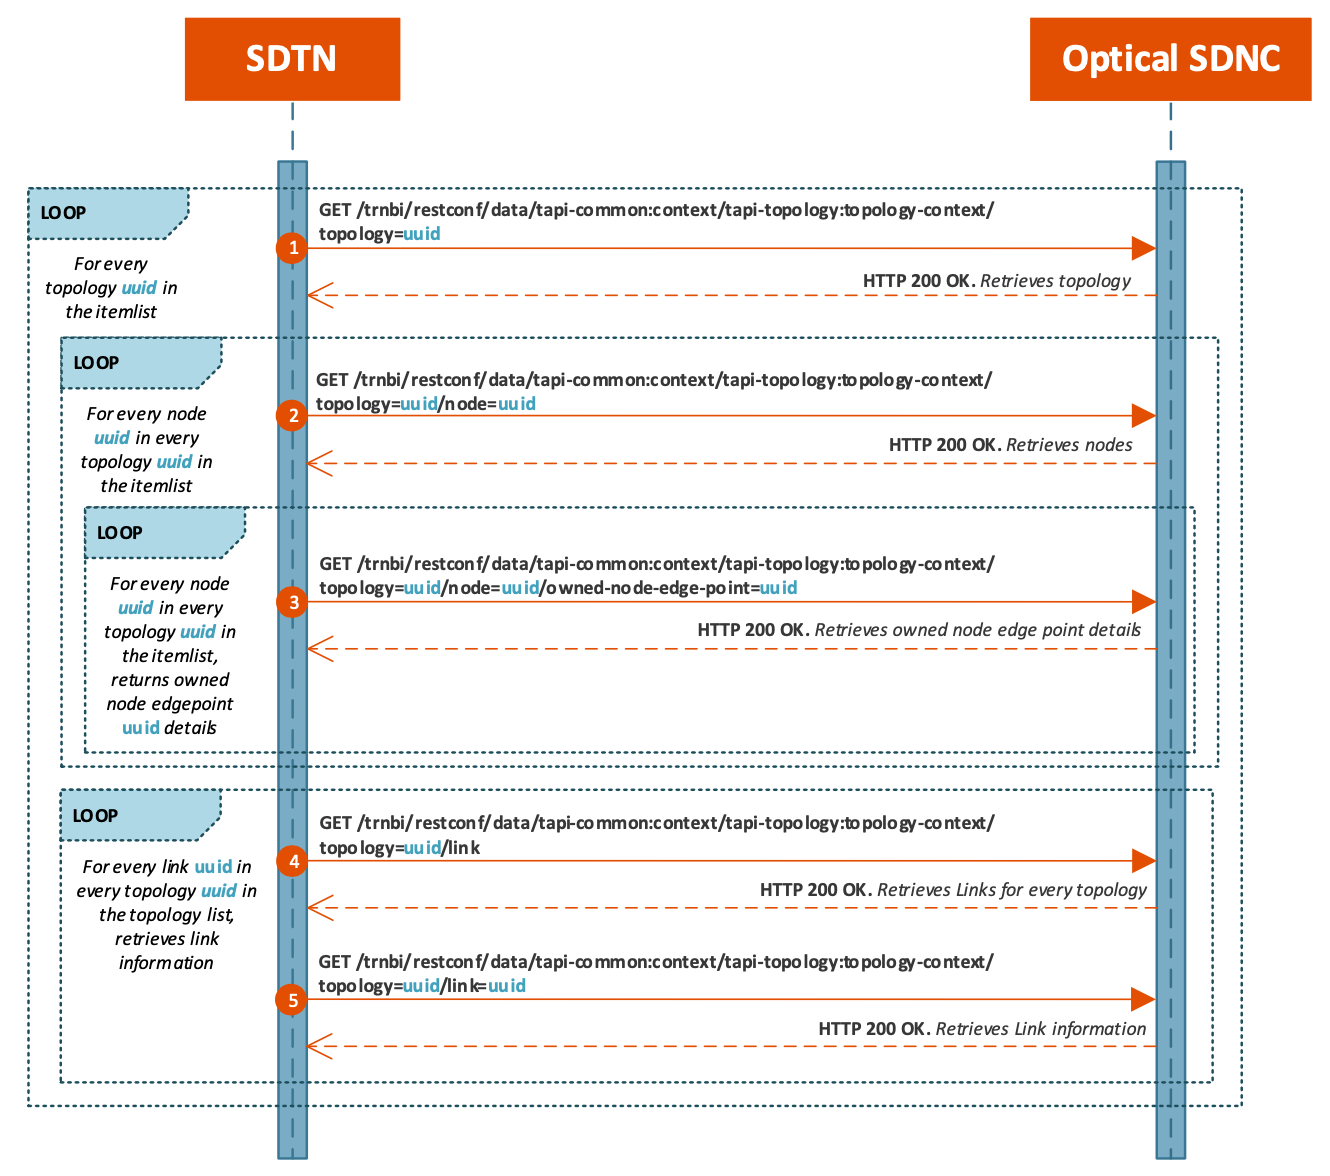
\includegraphics[width=\linewidth]{figs/optical_topology_workflow_2.png}
	\caption{Messages Interchanged for Optical Topology Discovery between the SDTN and Optical SDN-C}
	\label{FIG:optical_topology_workflow}
\end{figure}

Regarding the IP domain, to obtain the whole network topology, a query to the controller’s NBI to retrieve the network topologies available for all layers is sent; from here on, the client must perform per-layer queries to get more detailed information such as nodes, termination points of nodes, links, etc. \Cref{FIG:ip_topology_workflow} displays the RESTCONF-based queries in UML format for the topology retrieval in the IP domain. 
At this point, no inter-domain links were retrieved since there is no automatic mechanism supported on the domain controllers to expose information such as TTI (on the optical domain), LLDP (on the IP domain) or \texttt{Plug-id} (for both domains); therefore \texttt{Plug-id} based link discovery was simulated by adding user-defined \texttt{Plug-id} values to each port or at least to each domain edge port manually with the use of Python scripting. The inputted plug-id data was automatically detected by the SDTN and the inter-domain links between ports with matching \texttt{Plug-ids} were created, resulting in a complete multi-layer/multi-domain end-to-end topology as seen from the SDTN GUI.

%\begin{figure}
%	\centering
%		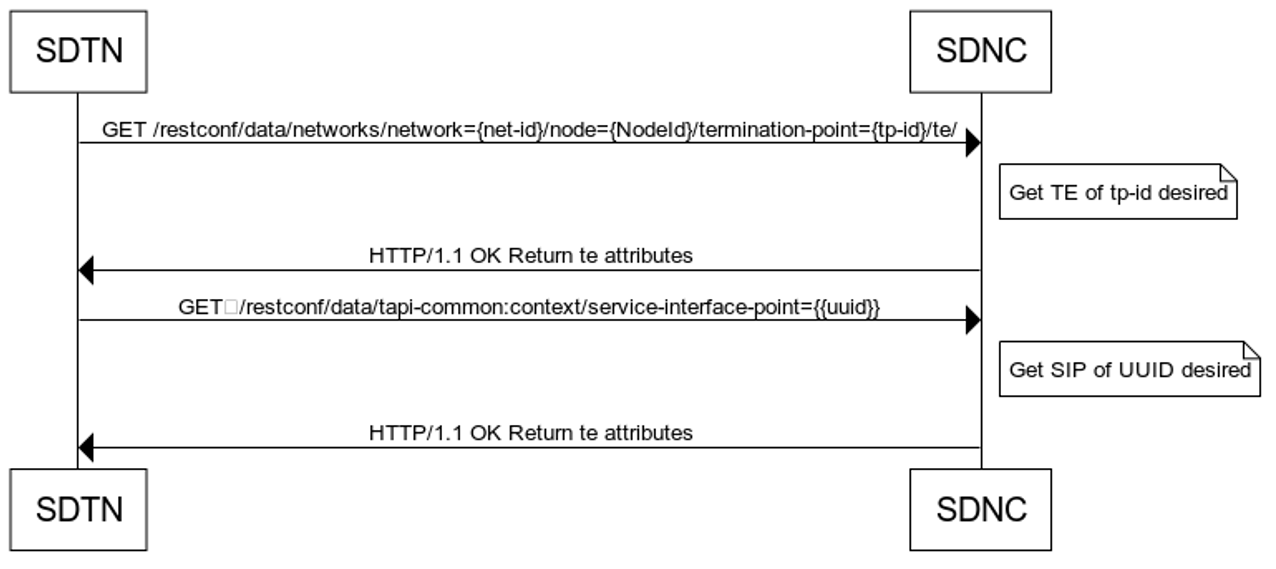
\includegraphics[width=\linewidth]{figs/topology_workflow.png}
%	\caption{Workflow for multi-layer topology SDTN-SDN-C}
%	\label{FIG:topology_workflow}
%\end{figure}

\begin{figure*}
	\centering
		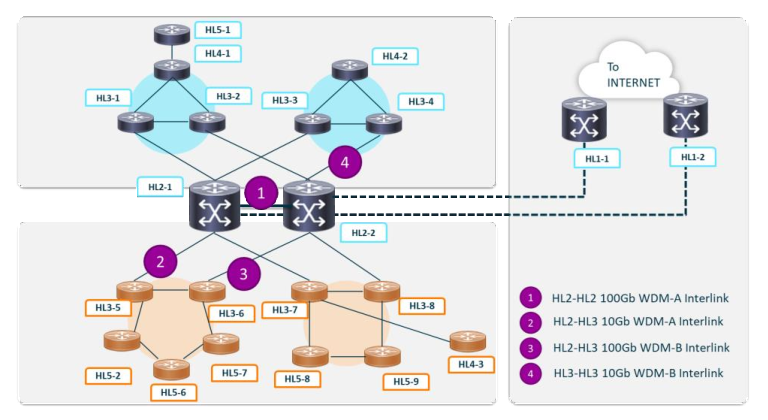
\includegraphics[scale=1]{figs/field_trial_environment_ip.pdf}
	\caption{Network Plane of the Field Trial Environment for IP/MPLS Testing and Evaluation}
	\label{FIG:field_trial_ip}
\end{figure*}

\begin{figure*}
	\centering
		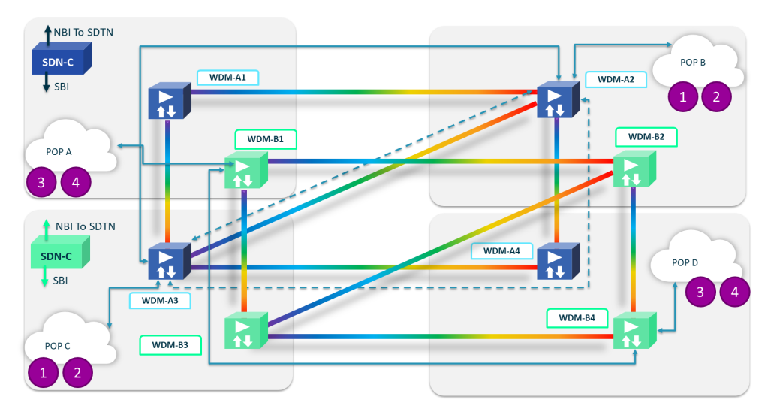
\includegraphics[scale=1]{figs/field_trial_environment_optical.pdf}
	\caption{Network Plane of the Field Trial Environment for Optical/WDM Testing and Evaluation}
	\label{FIG:field_trial_optical}
\end{figure*}

\subsection{Single-domain IP L2VPN provisioning}
\label{section:single-l2nm}

The L2VPN services are not exclusive of single domain implementations however due to implementation limitations in one of the SDN controller just the single domain L2VPN creation was tested. As described previously, in \ref{section:single-l2nm} In order to create the L2VPN service of the containers (SITE, VPN SERVICE) must be posted using the the following operations:

\begin{enumerate}
    \item Site creation. The two sites must be created on the SDN-C. Parameters such as \texttt{site-id} and \texttt{location-id}  must be provided.
    \item Service Creation (VPN-SERVICE). The identifier of the service (VPN-ID) and the Virtual Circuit Identifier \texttt{VC-ID} to be negotiated by the ends is provided.  
    \item Site Network Access Creation (SITE-NET-ACCESS). In this step all the data previously created is merged into a working L2VPN service to be deployed by the SDN-C on the devices using NETCONF. The configuration parameters needed on the body request for the SITE-NET-ACCESS creation includes: 
    \begin{itemize}
        \item \texttt{site-id}: Reference to customer site.
        \item \texttt{bearer-id}: Netowrk Interface used in the service.
        \item \texttt{vpn-id}: Reference to the VPN-SERVICE.
        \item IP connectivity, QoS management or Ethernet encapsulation
    \end{itemize}
\end{enumerate}

\begin{figure}
	\centering
		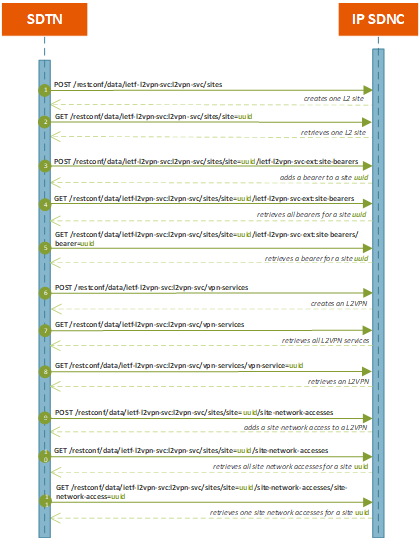
\includegraphics[width=\linewidth]{figs/l2sm_workflow_2.png}
	\caption{Messages Interchanged for L2VPN Provisioning between the SDTN and the IP SDN-C}
	\label{FIG:L2SM_workflow}
\end{figure}

The workflow between the SDTN and the IP controller has been summarized in the UML model presented on \cref{FIG:L2SM_workflow}. The four POST requests described previously, and their equivalent retrieval (GET) requests exchanged between the SDTN and the IP controller are included.

\section{Field Trial Environment for iFusion SDTN Demonstration}
\label{section:trial}

A field trial environment to demonstrate, test and evaluate the end-to-end multi-domain cases and the SDN-based iFusion Architecture was developed. It has two main layers: Firstly, a \hyperref[sec:contollay]{Control Layer} is comprised of two SDN IP domain controllers for a multi-vendor IP/MPLS network using an underlying WDM infrastructure and working in parallel with two SDN optical domain Controllers. On top of that, a multi\-layer, multi\-domain SDTN controller orchestrates the uses cases. Secondly, the \hyperref[sec:netlay]{Network Layer} is comprised of a Metropolitan WDM Network with N x 100G Lambda capacity providing interlink capabilities for a multi-domain IP/MPLS network following a hierarchical architecture that we denominate from HL1 (Hierarchical Layer No. 1) to HL5. We detail each of the layers in the next subsections. 

\subsection{Control Layer}
\label{sec:contollay}
A hierarchical SDTN architecture is built upon the reference design guidelines described in \cref{section:arq}. The key elements of the control layer are:
\begin{itemize}
    \item Infinera Transcend Maestro acting as SDTN controller.
    \item 2 x IP SDN-Cs, one for each cluster.
    \item 2 x Optical SDN-Cs, one for each cluster.
\end{itemize}

From the IP control perspective, SDN-Cs communicate with NEs via NETCONF/YANG and RESTCONF/YANG with SDTN.  On the other hand, from the Optical perspective, SDN-Cs follow a similar integration. At SBI, OpenROADM + OpenConfig models are used on top of NETCONF/YANG protocol. At NBI, a T-API v2.1 implementation is used.  

\subsection{Network Layer}
\label{sec:netlay}
We use a scale representation in terms of quantity of equipment, but a full network field trial with all the hierarchical layers that compose a real service provider deployment. In our notation and architecture, the IP/MPLS-base network is comprised of five (5) layer with the following responsibilities: 
\begin{itemize}
    \item HL1: Core P/PE-Routers acting as Toll Gates for interconnection of the Service Provider to the International Exit and using eBGP logical structure for publishing public IPv4/IPv6 prefixes to IP gates from and to a Tier-1/2 international Internet provider.
    \item HL2: Core P-Router responsible for the transportation of traffic between main cities and metropolitan areas sending/receiving traffic to HL1 interconnections from/to the International Internet.
    \item HL3: PE-Routers responsible for the aggregation and conglomeration of traffic from metropolitan and regional areas coming from network clusters and rings covering main and secondary cities for both fixed and mobile services.
    \item HL4: PE-Routers able to collect traffic from fixed access networks (DSLAM/CMTS/OLT) in metropolitan areas and high capacity corporate services. These are also able to collect traffic from mobile access networks coming from HL5 (former cell site routers) for generations 2G/3G/4G, 4.5G and new 5G in the near future.
    \item HL5: Provides connectivity access to corporations, enterprises, small businesses and mobile terminal nodes (BTS, NodeB, eNodeB) in remote areas. Formerly known as cell site routers in Mobile Service Providers, but now evolved and converged to serve multiple fixed plus mobile segments.     
\end{itemize}

The IP/MPLS network was built using seamless MPLS option-C. The network is organized by clusters and rings within. Each IP cluster groups devices of a specific vendor. The seamless MPLS signalling requires that an ingress PE-Router (originating HL4) from one cluster can establish an end-to-end LSP with a digress PE-Router (destination HL4), even if it belongs to a different cluster.”

Thus, the HL3 routers from each region establish an eBGP session with the Core-Routers (HL2). This session exports the Router-ID plus label information of all the routers in the region using BGP-LU \cite{rfc8277}. Additionally, there is another eBGP session between the HL3 of the region and the core Router-Reflectors to export the VPNv4 routes from each VPN service. This eBGP session requires a mandatory Next-Hop-Unchanged configuration to avoid network loops or misconfigured paths. All this control plane setup allows the creation of an end-to-end LSP from the access layer to the platforms without changing the configuration during the service provisioning.

Additionally, to deploy any of these services, the network has to fulfill the following basic requirements established between origin and destination:
\begin{itemize}
    \item PE connectivity based on IGP Router-ID/Loopback reachability.
    \item Label switching protocol enabled. MPLS and Labelling mechanism LDP, RVSP, other. 
    \item MP-BGP sessions between the PEs (address-family vpnv4/6, ipv4/6).
    \item Virtual Routing network instance. 
\end{itemize}

Four (4) IP/MPLS-based network links are transported by a two-vendor WDM underlying infrastructure. \Cref{FIG:field_trial_ip} depicts in purple the four interlinks 2 x 100G and 2 x 10G.  

Regarding the optical transport infrastructure, we have built a dual-plane independent metropolitan WDM network comprised of a ring of (4) four nodes each with N x 100G and N x 10G lambda capacity. \Cref{FIG:field_trial_ip} illustrates the optical WDM part of the field trial environment.


\section{Test Results}
\label{section:results}

Test results for the implementations of the Provision and Topology Network APIs and the SDTN controller’s integration with the SDN-C controllers in the Optical and IP domains are presented in this section. Two types of tests have been done in order to demonstrate orchestration functionalities in the multi-layer/multi-domain/multi-vendor network environment: 
\begin{itemize}
    \item Validate the compliance of the NBI implemented for each of the use cases.
    \item Validate the operative status of the configurations deployed in the network. 
\end{itemize}

\Cref{TAB:tested_use_cases} shows the use cases tested on the network scenario. These have been classified into three main categories based on the used cases defined: topology discovery, IP service provisioning and optical service provisioning. A general overview and the results obtained for each of them are approached individually in further subsections of this chapter. Regarding the single-domain use cases, results are shown independently for each vendor and for each network domain.

\begin{table*}
	\caption{List of Multi-Layer, Multi-Domain Tested Use Cases}
	\centering
		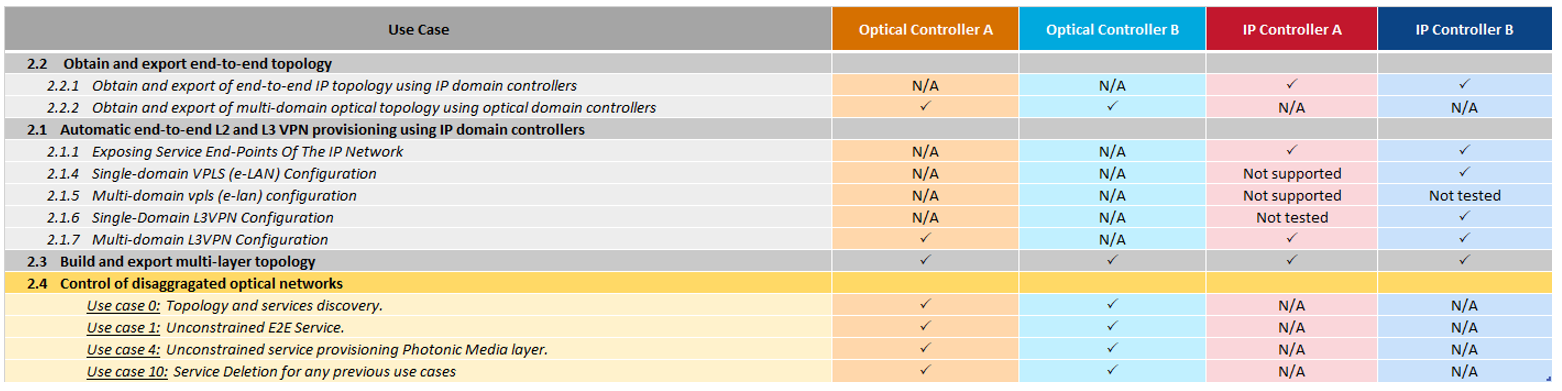
\includegraphics[scale=0.5]{figs/tested_use_cases.png}
	\label{TAB:tested_use_cases}
\end{table*}

\subsection{Multi-domain IP L3VPN provisioning}

Aiming to demonstrate the multi-domain/multi-vendor capabilities of the SDTN solution, a scenario for an L3VPN service configuration was proposed. The main goal was to create an L3VPN between two PE routers, each of them located in different IP domains. The IP domains are connected using a DWDM optical network, depicted in \cref{FIG:field_trial_optical}. The L3VPN service was created using the SDTN GUI and the configuration parameters used for this matter are shown in \cref{TAB:discovered_ip_l3vpn}.

\begin{table*}[]
\caption{Configuration Parameters for L3VPN}
\begin{adjustbox}{width=0.5\textwidth}
\small
\begin{tabular}{lll}
& \multicolumn{1}{c}{IP Vendor A} & \multicolumn{1}{c}{IP Vendor B} \\
{\color[HTML]{000000} NE IP Address} & {\color[HTML]{000000} 10.121.0.10}          & {\color[HTML]{000000} 10.120.1.52}     \\
\rowcolor[HTML]{F2F2F2} 
{\color[HTML]{000000} Hostname}            & {\color[HTML]{000000} 53-E114}              & {\color[HTML]{000000} 10.120.1.52}     \\
{\color[HTML]{000000} Description}         & {\color[HTML]{000000} SDTN\_TESTING-A}      & {\color[HTML]{000000} DEMO\_WORKSHOP} \\
\rowcolor[HTML]{F2F2F2} 
{\color[HTML]{000000} Service   Interface} & {\color[HTML]{000000} GigabitEthernet0/2/1} & {\color[HTML]{000000} 1/1/2}           \\
{\color[HTML]{000000} IP Address}          & {\color[HTML]{000000} 10.93.234.65/29}      & {\color[HTML]{000000} 10.93.233.65/29} \\
\rowcolor[HTML]{F2F2F2} 
{\color[HTML]{000000} VLAN   ID}           & {\color[HTML]{000000} 2020}                 & {\color[HTML]{000000} 999}             \\
{\color[HTML]{000000} VLAN Mode}           & \multicolumn{2}{c}{{\color[HTML]{000000} Dot1Q}}                                     \\
\rowcolor[HTML]{F2F2F2} 
{\color[HTML]{000000} VPN   ID}            & \multicolumn{2}{c}{\cellcolor[HTML]{F2F2F2}{\color[HTML]{000000} 15}} \\
{\color[HTML]{000000} VPN NAME}           & {\color[HTML]{000000} IP\_Nokia\_Huawei}                 & {\color[HTML]{000000} NA} 
\end{tabular}
\end{adjustbox}
\label{TAB:discovered_ip_l3vpn}
\end{table*}

\begin{figure}
	\centering
		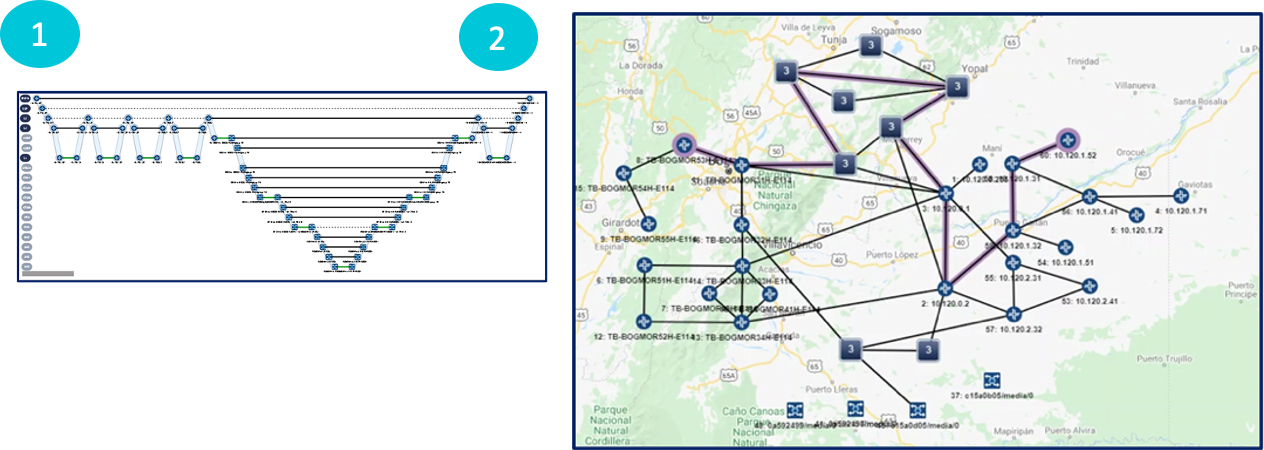
\includegraphics[width=\linewidth]{figs/l3vpn_results.png}
	\caption{L3VPN service creation results retrieved from the SDTN GUI. Included three visualization panes: The serivce details (Name, Topology, RD and Endpoint), the geographical view and the hop-by-hop connection view.}
	\label{FIG:l3vpn_results}
\end{figure}

The workflow between the SDTN and the IP controller has been summarized in the UML model presented on \cref{FIG:l3vpn_workflow}. This UML details, the procedure for creating the L3VPN from the SDTN GUI using the standard RESTCONF calls. 
\Cref{FIG:l3vpn_results} shows the three visualization options provided by the SDTN, each pane has the following information:
\begin{enumerate}
    \item The VPN service details including the service name, topology, and endpoint.
    \item The service route in the topology view, which includes the full path including the IP and optical devices comprised in the service.
    \item Layered view of the service. This view splits the service connections between layers, so the IP links connection is at the top. The Ethernet connections between routers are in the second layer and physical plus optical layers are decoupled in this hierarchical structure.
\end{enumerate}

\begin{figure}
	\centering
		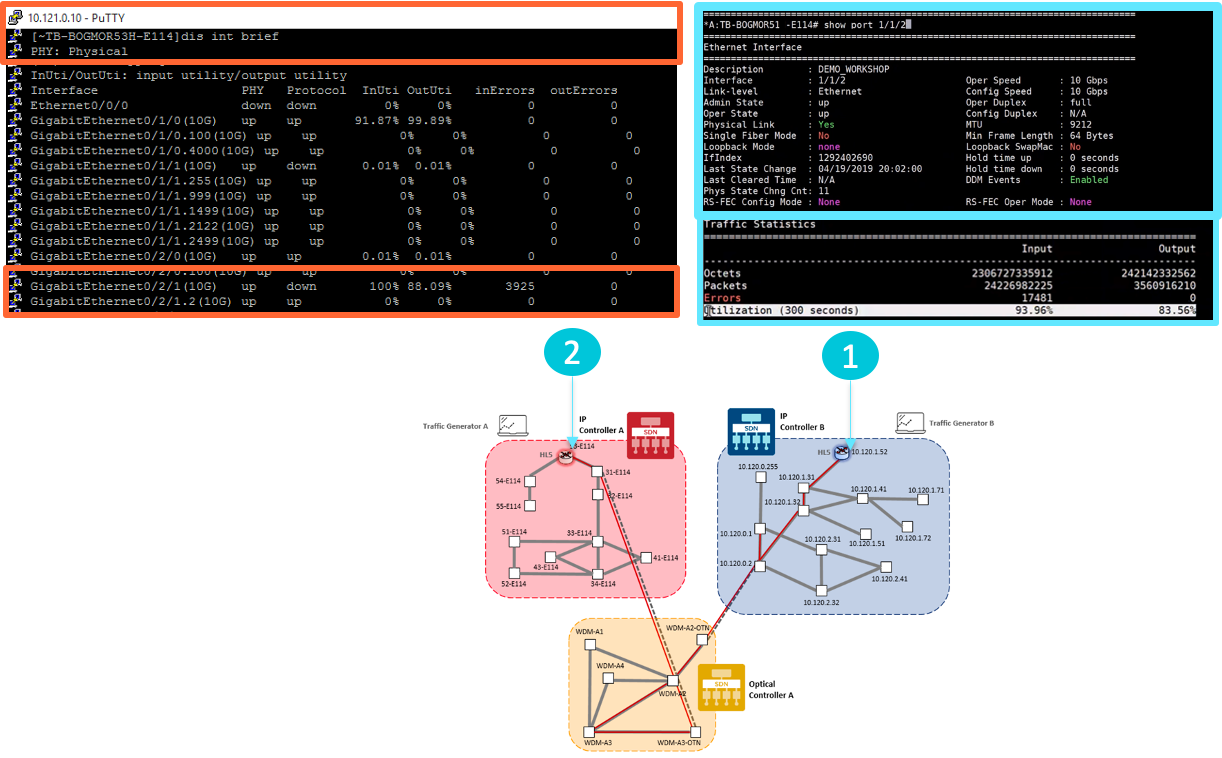
\includegraphics[width=\linewidth]{figs/counters.png}
	\caption{Traffic counters measured on the endpoints of the service. The utilization in both ends is close to 95\% due to the traffic injected by the generator.}
	\label{FIG:counters}
\end{figure}

The configuration of the IP L3VPN service in the network elements was verified by using their command line interface as well as the IP-SDN controller GUI. A traffic generator was used in site to introduce traffic on both ends of the network and test the functionality of the multi-domain L3VPN service created. \Cref{FIG:counters} shows the traffic statistics as seen on the command-line interface of the PE routers. In this figure, the two interfaces connected to the VPN services are selected, and their traffic counters are shown. The occupancy of the 10G ports is close to the 95\% during the test. 

\subsection{Multi-layer Topology Discovery \& Visualization}
Obtaining the end-to-end multi-layer and multi-domain topology via automatic network discovery is considered as a starting point towards the deployment of the SDTN multi-layer solution in the network scenario described in \ref{sec:netlay}. The first and most important step is for SDTN to discover all the network elements of the different domains by using the APIs provided by each of the IP and Optical controllers which implies the following steps:
\begin{enumerate}
    \item \textit{Enabling Network Adapters}: The network for each domain was discovered from the domain controllers individually by using domain adapters; each adapter uses the API provided by the domain controller to retrieve data such as nodes, inventories, termination points, links and services within it.
    \item \textit{Data Model Mapping}: The information model used in the domain controller's API is mapped into the SDTN model in order to harmonize the data across all domains, providing a per-layer view within both the inter-layer links and client-server relationships, thus resulting in a complete multi-layer view of the network and its services.
    \item \textit{Inter-domain links discovery}: End-to-end view of the whole network topology is formed by discovering the inter-domain links. Those interconnect the different vendors into a whole end-to-end multi-layer and multi-domain topology. There are many different mechanisms\footnote{TTI or plug-id for L0/L1, LLDP for L2 and IP address-based discovery for L3, among others such as alarm/statistics correlation with or without test data/circuits or inter-domain links simulation if no automatic mechanism is available} to achieve this purpose, such as TTI for OTU links, IP addresses for IP links, etc. If all the data required for full inter-domain and inter-layer link discovery is not reported by the third-party controllers, external data can be fed in via the SDTN NBI. 
\end{enumerate}

The number of discovered elements within the end-to-end network topology is summarized in \cref{TAB:discovered_elements}; for the optical domains in particular, the number of nodes for each topology correlates to the different layers, such as:
PHOTONIC\_MEDIA LAYER, DSR LAYER and ODU LAYER as defined in the YANG data model for T-API 2.1, hence the reason why there are more nodes retrieved other than those that are physically implemented in the testbed scenario. Additionally, the service interface points (SIPs) discovered for the optical domain are exposed in the controller NBI, making it easier for the SDTN to access these parameters and use them for future service provisioning. 

In the IP domain, however, given the different models implemented on the IP Controllers, the service end-points are not exposed to the SDTN SBI, which is why the interfaces and ports needed to be configured manually via Python scripting, a drawback when it comes to working with models that don’t follow a fully standardized model.

\begin{table*}[]
\caption{Discovered Network Elements for the Topology Visualization}
\begin{adjustbox}{width=1\textwidth}
\small
\begin{tabular}{lllll}
\hline
{\color[HTML]{000000} } &
  {\color[HTML]{000000} Optical Controller A} &
  {\color[HTML]{000000} Optical Controller B} &
  {\color[HTML]{000000} \begin{tabular}[c]{@{}l@{}}IP Controller A\end{tabular}} &
  {\color[HTML]{000000} IP Controller B} \\ \hline
{\color[HTML]{000000} \begin{tabular}[c]{@{}l@{}}Discovered nodes \\    (physical and logical)\end{tabular}} &
  {\color[HTML]{000000} 17} &
  {\color[HTML]{000000} } &
  {\color[HTML]{000000} 11} &
  {\color[HTML]{000000} 13} \\
{\color[HTML]{000000} \begin{tabular}[c]{@{}l@{}}Discovered links\\    (physical and logical)\end{tabular}} &
  {\color[HTML]{000000} 18} &
  {\color[HTML]{000000} } &
  {\color[HTML]{000000} 13} &
  {\color[HTML]{000000} 15} \\
{\color[HTML]{000000} Discovered service-end-points\footnote{The amount of end-points discovered for the domains not only comprehend those available for service provisioning, but all those available in the network }} &
  {\color[HTML]{000000} 97} &
  {\color[HTML]{000000} 90} &
  {\color[HTML]{000000} Not automatically discovered} &
  {\color[HTML]{000000} Not automatically discovered} \\
\rowcolor[HTML]{EFEFEF} 
{\color[HTML]{000000} Intra-domain IP links} &
  \multicolumn{4}{c}{\cellcolor[HTML]{EFEFEF}{\color[HTML]{000000} 2}} \\
{\color[HTML]{000000} Intra-domain Optical links (automatically discovered)} &
  \multicolumn{4}{c}{{\color[HTML]{000000} 4}} \\
\rowcolor[HTML]{EFEFEF} 
{\color[HTML]{000000} \begin{tabular}[c]{@{}l@{}}Inter-layer Inter-domain links
\end{tabular}} &
  \multicolumn{4}{c}{\cellcolor[HTML]{EFEFEF}{\color[HTML]{000000} 8}} \\ \hline
\end{tabular}
\end{adjustbox}
\label{TAB:discovered_elements}
\end{table*}



\subsection{Single-domain IP L2VPN provisioning}

\begin{figure}
	\centering
		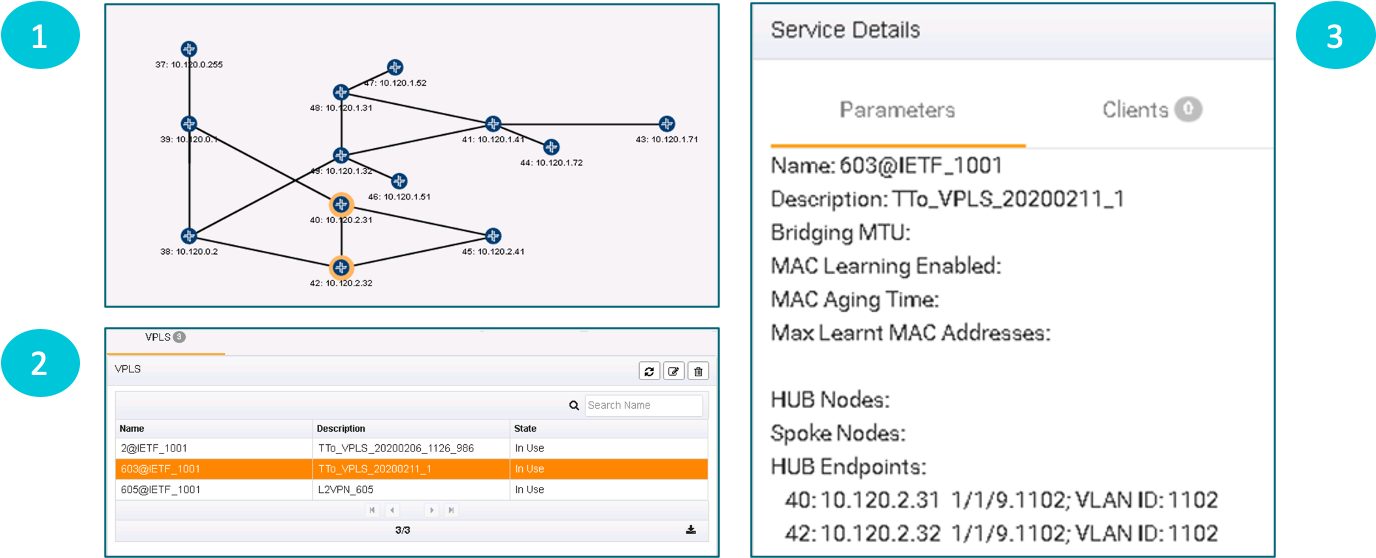
\includegraphics[width=\linewidth]{figs/l2vpn_results.png}
	\caption{L2VPN service creation results retrieved from the SDTN GUI. Information included three panes: Topology, Service lists and Service Details (Name, Topology and Endpoint).}
	\label{FIG:L2SM_results}
\end{figure}

This use case has been successfully tested using a single IP controller using the L2SM model to request service creation between the SDTN and the IP SDN controller. \Cref{FIG:L2SM_results} shows the L2VPN service creation results as seen from the SDTN GUI. The results has three information panes including the service details: 
\begin{itemize}
    \item Configured NEs in the network map. The yellow ones include the two service endpoints.
    \item List of all the services of a common type. In this case VPLS service was selected. 
    \item Service details, including: Name, Description and Endpoint (vlans, ports and topology-role). 
\end{itemize}

\subsection{Optical provisioning}
From the perspective of the optical networks, single domain unconstrained DSR connectivity services as well as Photonic Media Layer services were independently configured in both vendors’ DWDM networks and were verified in the respective NMS systems. The ONF T-API 2.1 YANG data model has been used for the query exchange between the SDTN HCO and the optical domain controllers given the support of this standard model in their NBIs. The UML diagram on \Cref{FIG:optical_provisioning_workflow} shows the HTTP POST request involved in the optical circuit creation as sent from the SDTN HCO towards the optical SDN-Cs, as well as the HTTP GET requests for information retrieval regarding particular connectivity services existing on the network. 

The DSR connectivity services created in both optical domains range from 1 GbE to 10 GbE and 100 GbE, all of them configured using the API Client as well as the SDTN HCO GUI. A total of 3 x 10 GbE and 4 x 100 GbE DSR connectivity services were provisioned simultaneously  in optical domain A, whereas given the network resources available in optical domain B, a 1G bE service as well as 2 x 10GbE services were provisioned. When it comes to photonic media-type services, 100 GbE and 200 GbE could be provisioned for optical domain A and B respectively. 

First, the API client was used to send the E2E DSR service creation query towards the SDN-Cs. For this, parameters\footnote{Parameters included in the body script for the service creation; other important ones include \texttt{service-interface-point}, \texttt{layer-protocol-name}, \texttt{service-layer} as well as the \texttt{service name} and a unique identifier \texttt{uuid}.} such as \texttt{service-interface-point}, \texttt{capacity} and the \\ \texttt{layer-protocol-qualifier} embedded in the POST body script needed to be correctly identified prior to sending the service creation petition, being that they depend strictly on the installed equipment and the resources available in the network, and therefore, when configured improperly, it led to the failure of the service creation or to  misconfiguration on the controller’s side. When sending the POST query from the SDTN HCO towards the optical controllers, an HTTP 202 accepted notification is returned by the SDN-C, meaning the controller has accepted the petition and would proceed with service creation; otherwise, an HTTP 400 bad request notification would be retrieved in case the petition was not accepted by the controller. 

\begin{figure}
	\centering
		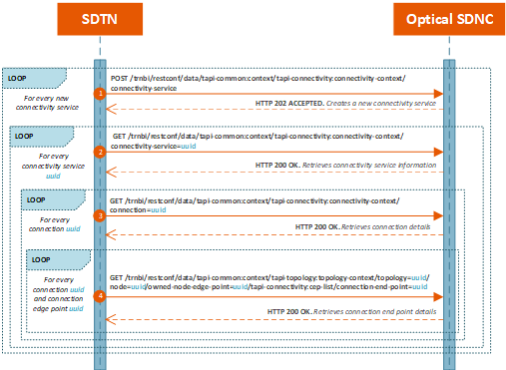
\includegraphics[width=\linewidth]{figs/optical_provisioning_workflow_2.png}
	\caption{Messages Interchanged for Optical Provisioning between the SDTN and the Optical SDN Controller}
	\label{FIG:optical_provisioning_workflow}
\end{figure}

\begin{figure}
	\centering
		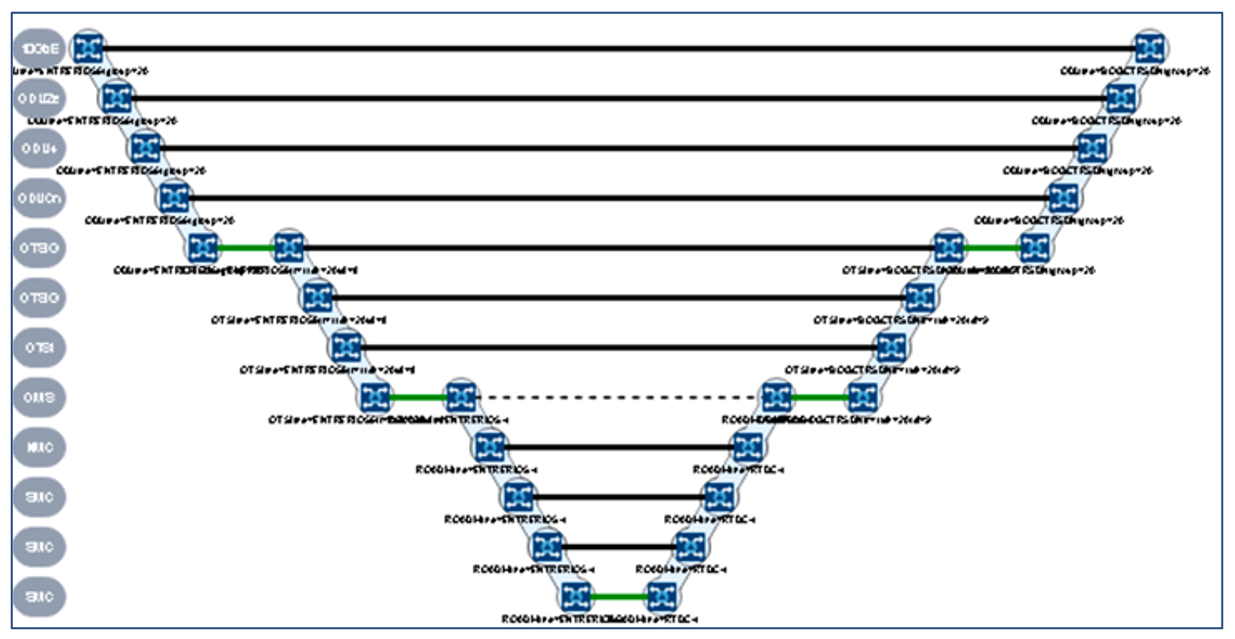
\includegraphics[width=\linewidth]{figs/optical_provisioning_result.png}
	\caption{Optical Provisioning Result for a Multi-Layer 10 GbE Service}
	\label{FIG:optical_provisioning_result}
\end{figure}

Additionally, from the API client tests, it was noted that even if both controllers are standards-based and implement T-API 2.1 in their NBIs, the modeling of some attributes is different from one another. From comparing the results retrieved via the API client, naming attributes for some of the objects\footnote{SIP\_NAME” in contrast to "INVENTORY\_ID", "CONN\_NAME" in contrast to "CONNECTION\_NAME", among others}, as well as the general modeling of the connections in regards of the route for an optical circuit, was noticed to be different. Likewise, the site names in one of the optical controllers did not coincide with the real name of the site but were based on an encoding made by the controller itself. Also, when using the SDTN HCO GUI to create the e2e connectivity services within the two network domains, this particular discrepancy was also visible via the multi-layer view of the services created, as seen on \cref{FIG:optical_provisioning_workflow}, where the different layers for a 1 GbE service are shown as exposed by the optical domain controller B, while on \cref{FIG:optical_provisioning_result} a multi-layer view of a 10 GbE service created in optical controller A is shown.


\section{Conclusions and Future Work}
\label{section:conclusions}
The foundation of the SDTN architecture is the data models themselves. RESTCONF/YANG aligned with IETF and ONF-based YANG models were preferred on the beginning of the integration between SDTN and the SDN-Cs  when the main focus was to use standardized APIs to access and retrieve the required information from the IP and optical controllers. It is the reason that in both optical domain controllers had been implemented ONF T-API 2.1 YANG models, making the integration process much easier; on the other hand, for the IP domain in particular, the usage of different pseudo-standard and reduced models was needed in order to execute the different test case scenarios. IETF YANG data models for the IP world still require additional efforts to fit in all the MPLS-based use cases to improve their synergy. 

A brief summary of the issues faced during the integration of the SDTN architecture, as a reference point to another work or future work: 

\begin{itemize}
    \item Connectivity, latency and internal processing times between the HCO and some of the SDN-Cs can impact the integration and result in miscommunication, creating the timeout of SDN transport protocols, i.e., RESTCONF and NETCONF.  
    \item \textit{Ghost} objects that are not completely deleted in the controllers can lead to misunderstanding in the topology construction. 
    \item The unsolicited data retrieved by a lack of standardization or a bias in the implementation of the standards can lead to uncompleted transactions or loops in execution tasks.
    \item Absence of data in the SDN domain controllers for an automatic inter-domain link discovery.
    \item Differences in the RESTCONF/YANG implementations on the SDN Controllers. Even if the YANG models were the same, the parameter translation between NBI and SBI can restrict some configurable parameters (i.e., max length size of a description field) and may generate implementation differences. This would result in possible errors during the execution of the creation process.
    \item Differences in the RESTCONF/YANG error handling. A set of well-defined error codes is mandatory in the hierarchical architecture.
\end{itemize}

However, except for the lack of the inter-domain port exposure on the IP domains as well as the retrieval of data required for automatic discovery of inter-domain links (e.g., \texttt{Plug-ID} and TTI values), the APIs provided sufficient functionality for their implementation of all the use cases approached for this paper, demonstrating the viability of the SDTN solution on a multi-vendor, multi-layer and multi-domain network environment.

\subsection{Future Work}
As future work, the hybrid SDN deployment done until now must be complemented with an integration between the NBI exposed by the SDTN and the OSS application ecosystem. The OSS ecosystem can include, for example, strategic and tactical planning applications, able to support the year by year demand management and planning tasks done within the organization. A common interface defined and available for these tasks would allow the OSS system providers to focus on the quality of the applications developed, forgetting the complexity of network management. Economically it will generate direct reductions in application integration time.

Additionally, the scope of this work can be extended to cover traffic engineering use cases. Standardization in the NBI requests to support LSP creation will enable easy management of the traffic flows in the network, generating a real massification of the traffic engineering deployment and creating new network optimization solutions for the operators.

\printcredits

\section*{Acknowledgements}
This work has been supported by Telefonica I+D as part of the Fusion, iFusion and OpenFusion projects. The authors would like to thank all the SDN technical teams and leaders that participated in the development, deployment and testing of this SDTN architecture. Many thanks for their contributions to Manuel Santiago, Gloria Gomez, Julia Rodriguez and Zdravko Stevkovski from Infinera; Randy Quimbay and David Rocha from Telefonica Colombia; and Andrea Valencia, Juan Suarez, Juan Agredo and Daniel Hernandez from Wipro Limited.   


%% Loading bibliography style file
%\bibliographystyle{model1-num-names}
%\bibliographystyle{cas-model2-names}
\bibliographystyle{ieeetr}

% Loading bibliography database
\bibliography{bibliography}


%\vskip3pt

\bio{figs/1010179793S.jpg}
Samier Barguil (M.Sc. 2018). PhD Candidate from the Universidad Autonoma de Madrid. Electronic Engineer from the District University of Bogot\'a Franscisco Jos\'e de Caldas and Master in Science in Industrial Automation of the Universidad Nacional de Colombia. Currently is the IP SDN Technical Leader at Wipro Technologies Ltd. 
\endbio


\bio{figs/victor.jpg}
Víctor López (M.Sc. 2005 - Ph.D. 2009) is a Technology Expert at Systems and Network Global Direction in Telefónica gCTIO. He works on the global IP and transport processes of the Telefonica group. He serves as co-chair at the Open Optical Packet Transport group in the Telecom Infra Project. He has co-authored more than 200 publications, six patents and contributed to IETF and ONF. Moreover, he is the editor of the book Elastic Optical Networks: Architectures, Technologies, and Control (308 pages, Springer 2016). His research interests include the integration of Internet services over IP/MPLS and optical networks and control plane technologies (PCE, SDN, GMPLS).
\endbio

\bio{figs/cristyan_manta.jpeg}
Cristyan Manta-Caro (M.Sc. 2007 - PhD (c)) currently serves as Solutions Manager and Managing Consultant at Wipro Technologies Ltd within the Comms EGM BU. He is responsible for structuring and leading transformation projects for Digital and Telecommunications providers. With over 15 years of experience in managing, optimizing, analyzing telecommunications and Information Technology IT infrastructures with primary vendors and CSP. He received his Master of Science and Electronics Engineering degree from the District University of Bogota Francisco Jos\'e de Caldas. His research interests include SDN architectures, Future Internet, DevNet \& NetDevOps, Cloud Technologies for IoT and the Web of Things WoT.
\endbio

\bio{figs/cristian_rosero.jpg}
Cristian Rosero Carvajal is an Electronics Engineer from Cali (Colombia) currently based in Bogotá. He is a passioned for everything from Software, Coding, DBA systems, Virtualization, Networking, Transmission, Research, Web design to development. He has 7+ years of working experience as a Networking and Transmission engineer and now as an SDN WDM Planner at Wipro Technologies Ltd in this new service provider World. Researcher and consultant in software algorithms, data models and DBA systems. He is oriented to process re-engineering and improvement through data science and his spirit of artistic awareness applied to engineering.
\endbio

\bio{figs/Edward_Echeverry_v2.jpg}
Edward Echeverry is Head Of Transport (IP and Optical Network) in Telefonica Colombia. Electronic Engineer, Telecommunications Specialist with a 15+ years of experience in the field. High technical skills and advanced experience in the design, planning and implementation of 3G/4G mobile, IP/MPLS and new generation optical networks, as well as in management and deployment of projects. Lead PoC concept tests of an end-to-end SDTN system including the different layers of IP \& Optical transport network that allowed us to define the use cases of topology and services L1/L2/L3. The tests looked at the use of SBI/NBI T-API IETF-Based interfaces. His research interests include emerging network automation technologies and SDTN architectures.
\endbio

\hfill\break
\hfill\break
\hfill\break
\hfill\break

\bio{figs/arturomayoral.png}
Arturo Mayoral López de Lerma is a Technology Expert in Transport Networks at the Global Systems \& Network department of Telefónica GCTIO. He received the Ph.D. degree in telecommunications engineering from the Universitat Politècnica de Catalunya (UPC) in 2019. His  research  interests  include  optical network design and Software Defined Networking (SDN). He is author or co-author on over 50+ journals and conference papers.
He graduated in Telecommunications Engineering by the Universidad Autónoma de Madrid in 2013 and he started his professional career in 2012, as undergraduate researcher in Telefonica I+D (R\&D) where developed his Final Career’s Project, awarded with the Best Final Project Prize by the Official College of Telecommunication Engineers (COIT).
\endbio

\bio{figs/ogondio.png}
Óscar González de Dios received his M.S. degree in telecommunications engineering and Ph.D. degree (Hons.) from the University of Valladolid, Spain. He has 19 years of experience in Telefonica I+D, where he has been involved in a number of European research and development projects (recently, STRONGEST, ONE, IDEALIST, and Metro-Haul). He has coauthored over 100 research papers and 10 IETF RFCs. He is currently the head of SDN Deployments for Transport Networks, Telefonica Global CTIO. His main research interests include photonic networks, flexi-grid, interdomain routing, PCE, automatic network configuration, end-to-end MPLS, performance of transport protocols, and SDN. He is currently active in several IETF Working Groups and is the Co-Chair of TIP CANDI WG.
\endbio

\bio{figs/juan_pedro.png}
Juan Pedro Fernández-Palacios Giménez received the MS in Telecommunications Engineering from Polytechnic University of Valencia in 2000. In Sept. of 2000 he joined Telefonica I+D where his research activities where focused on the design of new data and control plane architectures for IP over optical networks. He is author of 6 patents filled in Europe and US and more than 70 publications in conferences and journals. He was coordinator of two European research projects on optical transport networks (MAINS and IDEALIST) between 2011 and 2014. In 2013 he joined the Telefonica Global CTO office as Head of Transport. In 2016, he also took this position in Telefonica-O2 Germany. Since June 2017 he is leading the Integrated Transport Centre, a global organization in Telefonica in charge of defining the strategic network planning and technology for IP, DWDM, MW and satellite networks
\endbio

\bio{figs/jutta_685x685.jpg}
Jutta Kemppainen received her Master of Science (Tech.) in 1999 from Helsinki University of Technology (now part of Aalto University). She works as Senior Principal Product Manager at Infinera, managing Infinera multi-layer, multi-domain and multi-vendor transport network automation solutions. She has over 20 years of experience of telecommunications software automation products and has been concentrating on Software-Defined Networking (SDN)-based solutions in the last 7+ years. During this time Kemppainen has been co-operating with 70+ network providers, including many of the largest and technically most advanced in the industry, in designing and defining requirements for practical transport network automation solutions.
\endbio

\bio{figs/janne_karvonen_640x640.jpg}
Janne Karvonen (M.Sc.(Tech.) 1993 Helsinki University of Technology) is a Senior Software Architect at Infinera Corporation. He works in the Systems Architecture Group, focusing on Software Defined Networking Technologies and IP/MPLS Network Management Systems. He has over 30 years of experience in Software Engineering and more than 20 years of experience in Telecommunications Network Management Systems, covering both optical and packet based technologies. His research interests include SDN technologies for multi-layer, multi-domain and multi-vendor networks, with special focus on SDN API technologies, Multi-Layer Path Computation Algorithms and utilization of Machine Learning in SDN networks.
\endbio

\bio{figs/natalia_maya.png}
Natalia Isabel Maya Perfetti is an Electronics and Telecommunications engineer graduated from Universidad del Cauca, Colombia back in 2018; thence, she has been working as a network planning engineer in Infinera Colombia where she supports different tasks related to DWDM Network Planning. For the last year she has also been responsible for the testing of the SDTN solution in the field trial environment.
\endbio

\end{document}

